% ==============================================================================
\chapter{Active edge sensors}
\label{ch:ActiveEdgeSensors}
% ==============================================================================    

Active-edge technology allows for seamless tiling of pixel sensors by
depleting the sensors up to their physical edges. This allows for high
coverage without creating overlaps between the pixel sensors and
therefore reduces the material budget in the detector. The process
consists of extending the backside implantation to the edge.

This technology is particularly interesting for the CLIC vertex
detector where the material budget is constrained to be only
$0.2\%$~X\textsubscript{0} per layer. Ladders of pixel detectors can
be made without overlaps and with a high coverage.

In this chapter, the fabrication process for active edge sensors is
described. Planar sensors produced by Advacam~\cite{AdvacamRef} and
bump bonded to Timepix3 ASICs are tested in test beams. The signal
collection and the efficiency at the edge are presented. Test beam
results are compared to TCAD simulations.

%% --------------------------------------------- %%
\section{The active-edge technology processing}

Thin $50-150\,\micron$ thick n-in-p planar sensors with active edges
have been produced by Advacam~\cite{AdvacamRef} using a Deep Reactive
Ion Etching (DRIE) process. The DRIE process is used to make trenches
around the sensors and allows for extending the back-side
implantation, and thereby the bias voltage, to the edge of the sensor
by doping the sensor sides. The gradient of potential between the edge
and the last pixel can be very high and could lead to a breakdown of
the sensor. A guard ring (GR) consists of an n-implant with a metallic
contact on top of it surrounding the pixel matrix close to the edge
and thereby smoothening the potential transition between the edge and
the neighbouring pixels. The guard ring can be kept floating or
grounded by connecting it to the ground potential of the readout ASIC.

The active-edge sensors are bump bonded to Timepix3 readout chips
($55\,\micron$ pixel pitch) and studied in test beams and
simulations. A list of produced assemblies is given in
\cref{tab:ActiveEdgeAssemblies}. These assemblies are the same as the
ones studied in \cref{ch:FE_electronics} and
\cref{ch:ThinSensorsStudies}. In this chapter we focus on their edges.

Timepix3 ASICs provide an extra row of grounded pixels allowing to
connect the guard ring to ground
potential. Figure~\ref{fig:activeedge} shows a cross section of an
active-edge sensor with and without guard ring.

\begin{table}[htbp]
  \centering
  \caption{Details of different Advacam planar pixel sensors
    bump-bonded to Timepix3 readout ASICs. The edge distance is
    defined by the distance between the last pixel implant and the
    physical sensor edge.}
  \label{tab:ActiveEdgeAssemblies}
  \resizebox{\textwidth}{!}{\begin{tabular}{lccccc}
    \toprule
    Assembly & Thickness [\micron] & Type & Edge distance [\micron] &
                                                                      Guard-ring potential & Timepix3 ID \\
    \midrule
      20-NGR-50 & 50 & n-in-p & 20 & Without GR & W19\_G7 \\
     23-FGR-50  & 50 & n-in-p & 23 & Floating & W19\_F7 \\
     28-GNDGR-50  & 50 & n-in-p & 28 & Grounded & W19\_L8 \\
     55-GNDGR-50 & 50 & n-in-p & 55 & Grounded & W19\_C7 \\ \hline
     55-GNDGR-100 & 100 & n-in-p & 55 & Grounded & W5\_E2 \\ \hline
     55-GNDGR-150  & 150 & n-in-p & 55 & Grounded & W5\_F1 \\ %% \hline
     %% W2\_J5 & 300 & p-in-n & - & - & - \\
    \bottomrule
  \end{tabular}}
\end{table}


\begin{figure}[htbp]
  \centering
  \begin{subfigure}[b]{0.45\textwidth}
    \begin{tikzpicture}
      \node[anchor=south west,inner sep=0] (image) at
      (0,0){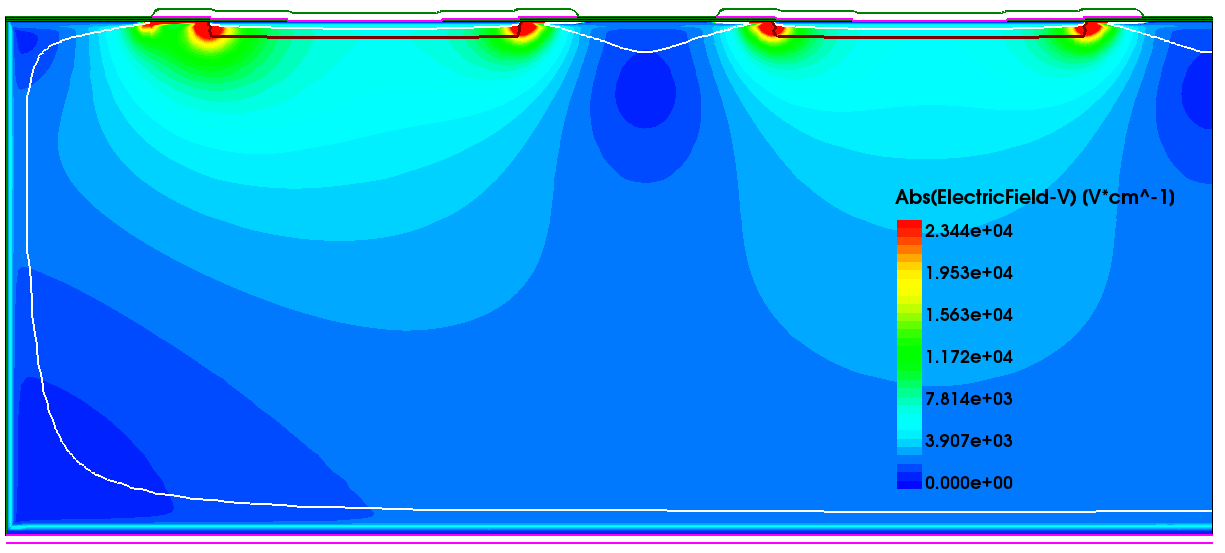
\includegraphics[width=\textwidth]{figures/ActiveEdge/Efield_20_NGR.png}};
      \begin{scope}[x={(image.south east)},y={(image.north west)}]
        \draw[-, dashed, line width=.7pt, color=white](0.1, 0.05) -- (0.1, 0.92);
        \draw[-, dashed, line width=.7pt, color=white](0.54, 0.05) -- (0.54, 0.92);
        
        \draw[<->, line width=.7pt, color=black](0.01, 1) -- (0.16, 1); % edge width
        \node[above, color=black] at (0.05, 1) {edge};
        
        \draw[<->, thick, color=black](0.17, 1) -- (0.43, 1); % n-implant
        \node[above, color=black] at (0.33, 1) {n-implant};

        \node[above, color=white] at (0.3, 0.5) {\textbf{p-substrate}};
        \draw[<->, thick, color=black](0.54, 0.0) -- (0.98, 0.0); % pixel width
        \node[below, color=black] at (0.75, 0.0) {pixel (55 \micron)};
        
        \draw[-, line width=3pt, color=violet](0.0, 0.05) -- (0.98, 0.05); % p+ backside contact
        \node[below, color=violet] at (0.15, 0.0) {p+ backside contact};
        \draw[-, line width=3pt, color=violet](0.0, 0.045) -- (0.0, 0.93); % p+ active-edge contact
        \node[left, color=violet, rotate=90] at (-0.05, 0.7) {p+ active edge};
        % \node[left, color=white, rotate=90] at (0.08, 0.9) {\textbf{final pixel edge}};

        % \draw[help lines,xstep=.1,ystep=.1] (0, 0) grid (1,1);
        % \foreach \x in {0,1,...,9} { \node [anchor=north] at (\x/10,0) {0.\x}; }
        % \foreach \y in {0,1,...,9} { \node [anchor=east] at (0,\y/10) {0.\y}; }

      \end{scope}
    \end{tikzpicture}
    \caption{No guard ring}
  \end{subfigure}\hfill
  \begin{subfigure}[b]{0.45\textwidth}
    \begin{tikzpicture}
      \node[anchor=south west,inner sep=0] (image) at
      (0,0){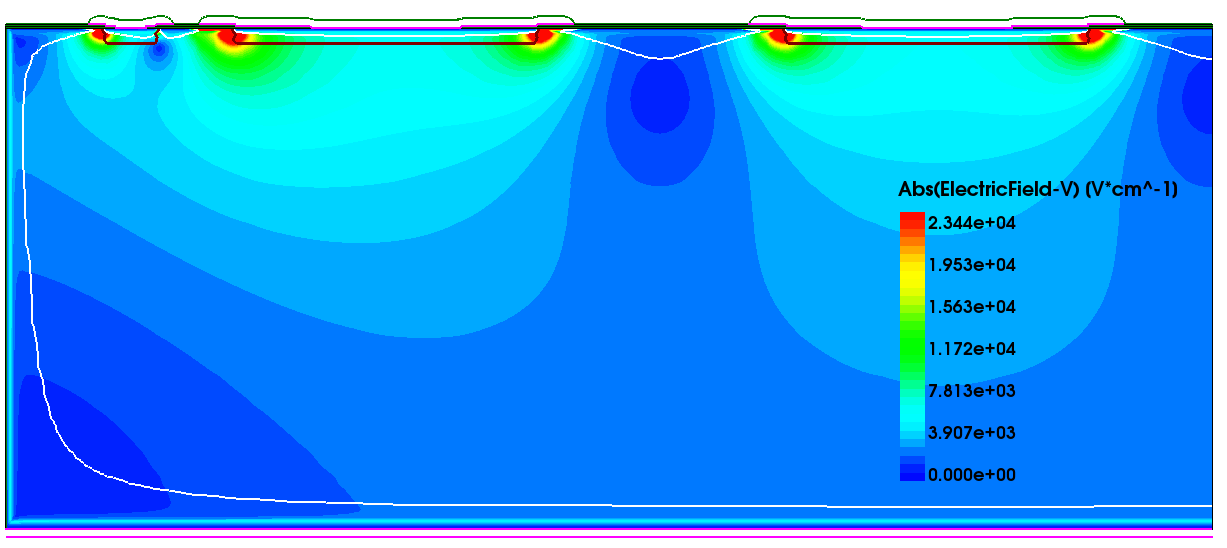
\includegraphics[width=\textwidth]{figures/ActiveEdge/Efield_23_FGR.png}};
      \begin{scope}[x={(image.south east)},y={(image.north west)}]
        \draw[-, dashed, line width=.7pt, color=white](0.14, 0.05) -- (0.14, 0.92);
        \draw[-, dashed, line width=.7pt, color=white](0.54, 0.05) -- (0.54, 0.92);
        \draw[<->, line width=.7pt, color=black](0.01, 1) -- (0.16, 1); % edge width
        
        \node[above, color=black] at (0.1, 1) {edge};
        \node[above, color=white] at (0.1, 0.75) {\textbf{GR}};
        \node[above, color=white] at (0.3, 0.5) {\textbf{p-substrate}};
        \draw[<->, line width=.4pt, color=black](0.54, 0.0) -- (0.98, 0.0); % pixel width
        \node[below, color=black] at (0.75, 0.0) {\small{pixel (55
            \micron)}};

        \draw[<->, thick, color=black](0.19, 1) -- (0.44, 1); % n-implant
        \node[above, color=black] at (0.33, 1) {n-implant};
        
        \draw[-, line width=3pt, color=violet](0.01, 0.05) -- (0.99, 0.05); % p+ backside contact
        \draw[-, line width=3pt, color=violet](0.01, 0.045) -- (0.01, 0.95); % p+ active-edge contact
        % \draw[help lines,xstep=.1,ystep=.1] (0, 0) grid (1,1);
        % \foreach \x in {0,1,...,9} { \node [anchor=north] at (\x/10,0) {0.\x}; }
        % \foreach \y in {0,1,...,9} { \node [anchor=east] at (0,\y/10) {0.\y}; }
      \end{scope}
    \end{tikzpicture}
    \caption{With guard ring}
  \end{subfigure}
  \caption{Schematic showing the cross section of a $50\,\micron$
    thick sensor with active-edge technology. The pixel grid
    considered in the analysis is indicated with dashed lines. The
    electric field distribution obtained from a TCAD simulation with a
    bias voltage of 15~V is also illustrated. (a) does not contain any
    guard ring (GR) and (b) contains a guard ring at the edge.}
  \label{fig:activeedge}
\end{figure}

%% --------------------------------------------- %%
\newpage
\subsection{Process flow for sensor production by the manufacturer}
\label{sec:AdvacamProcessFlow}

The process flow used by the manufacturer to produce active-edge
n-in-p sensors is schematically illustrated in
\cref{fig:AdvacamProcessFlow} and described as
follows~\cite{AdvacamProcessFlow}.

\begin{enumerate}[label=(\alph*)]
\item First, the backside implantation is done by doping the detector
  wafer with borons.
\item The wafer is then bonded to a support wafer to perform the next
  steps.
\item By grinding and CMP (Chemical-mechanical planarisation)
  polishing the final detector thickness is obtained.
\item The doping for the pixels and also the guard rings are implanted
  with phosphorus ions.
\item The DRIE etching is performed to uncover the edges of the
  detector.
\item Phosphorus ions are implanted to the sidewalls of the sensor to
  activate the edges.
\item Annealing of the sensor in order to activate the dopants and
  oxidation of the edges.
\item The opening of the contacts for the Aluminum patterning and the
  deposition of the UBM layer for the pixels and guard rings.
\item The support wafer is finally removed and the backside metal is
  deposited. The sensor is ready to be bump bonded to the readout
  chip.
\end{enumerate}


\begin{figure}[htbp]
  \centering
  \begin{subfigure}[b]{0.3\textwidth}
    \centering
    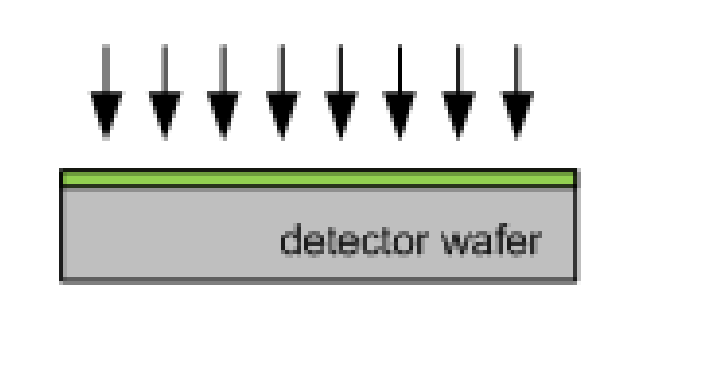
\includegraphics[width=\textwidth]{figures/ActiveEdge/advacamProcess/wafer_1.pdf}
    \caption{}
  \end{subfigure}\hfill
  \begin{subfigure}[b]{0.3\textwidth}
    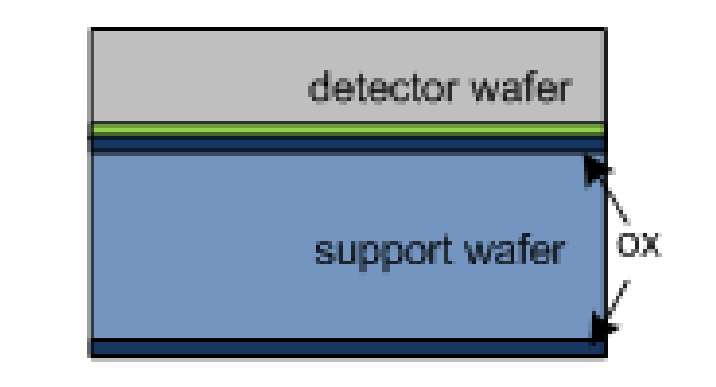
\includegraphics[width=\textwidth]{figures/ActiveEdge/advacamProcess/wafer_2.pdf}
    \caption{}
  \end{subfigure}\hfill
  \begin{subfigure}[b]{0.3\textwidth}
    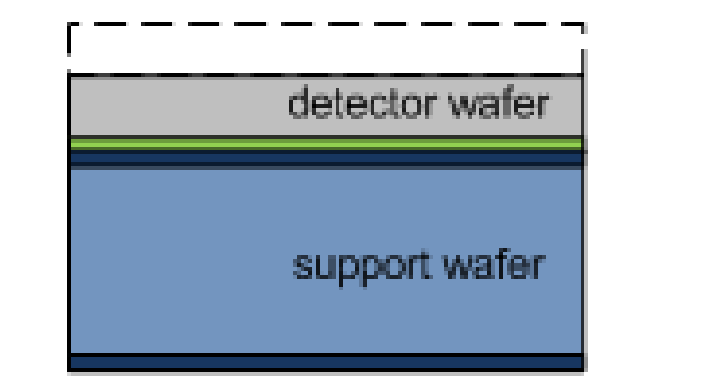
\includegraphics[width=\textwidth]{figures/ActiveEdge/advacamProcess/wafer_3.pdf}
    \caption{}
  \end{subfigure}\\

  \begin{subfigure}[b]{0.3\textwidth}
    \centering
    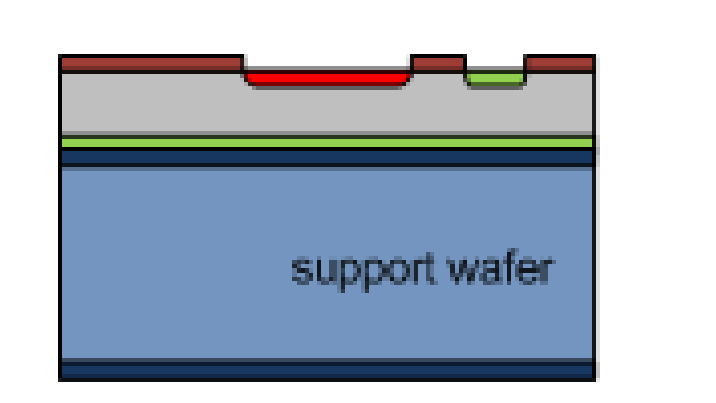
\includegraphics[width=\textwidth]{figures/ActiveEdge/advacamProcess/wafer_4.pdf}
    \caption{}
  \end{subfigure}\hfill
  \begin{subfigure}[b]{0.3\textwidth}
    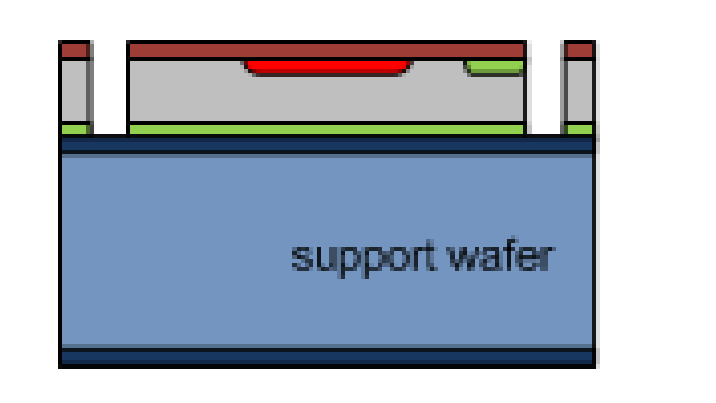
\includegraphics[width=\textwidth]{figures/ActiveEdge/advacamProcess/wafer_5.pdf}
    \caption{}
  \end{subfigure}\hfill
  \begin{subfigure}[b]{0.3\textwidth}
    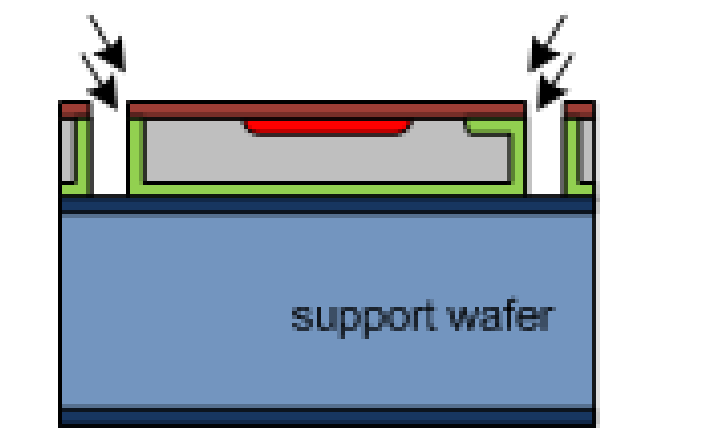
\includegraphics[width=\textwidth]{figures/ActiveEdge/advacamProcess/wafer_6.pdf}
    \caption{}
  \end{subfigure} \\

  \begin{subfigure}[b]{0.3\textwidth}
    \centering
    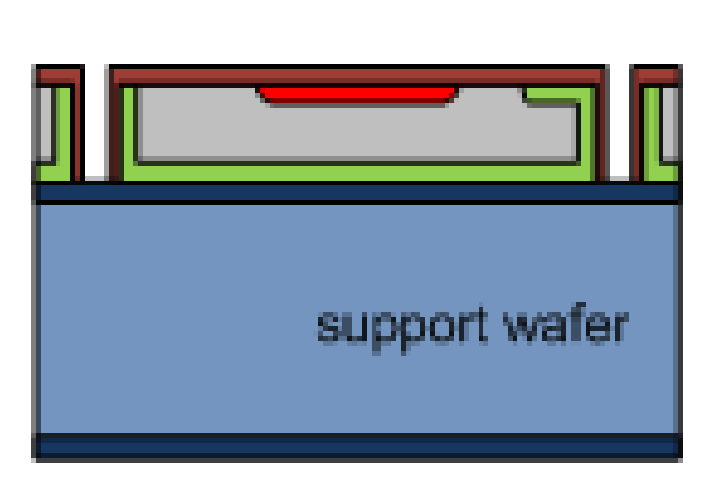
\includegraphics[width=\textwidth]{figures/ActiveEdge/advacamProcess/wafer_7.pdf}
    \caption{}
  \end{subfigure}\hfill
  \begin{subfigure}[b]{0.3\textwidth}
    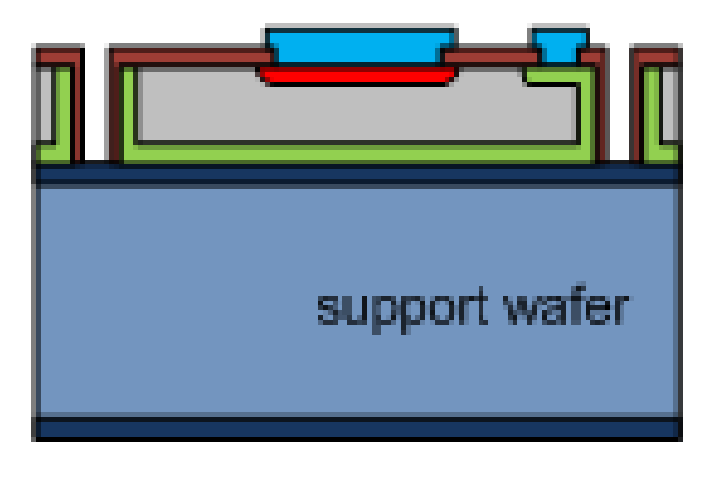
\includegraphics[width=\textwidth]{figures/ActiveEdge/advacamProcess/wafer_8.pdf}
    \caption{}
  \end{subfigure}\hfill
  \begin{subfigure}[b]{0.3\textwidth}
    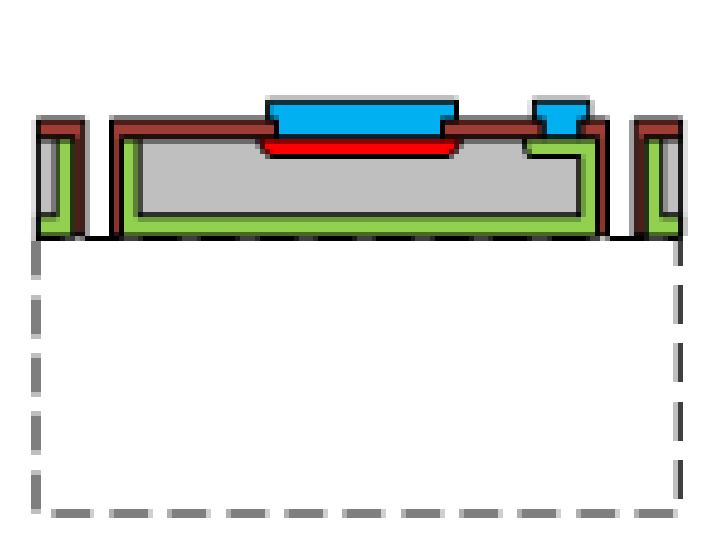
\includegraphics[width=\textwidth]{figures/ActiveEdge/advacamProcess/wafer_9.pdf}
    \caption{}
  \end{subfigure}

  \caption{Schematic illustration of the process flow for the
    fabrication of planar n-in-p active edge sensors by the
    manufacturer~\cite{AdvacamRef}.}
  \label{fig:AdvacamProcessFlow}
\end{figure}


%% --------------------------------------------- %%
\newpage
\subsection{Layout parameters of produced assemblies}
\label{sec:AEgeometry}


\cref{tab:ActiveEdgeAssemblies} shows the assemblies tested in
test-beam campaigns at the CERN SPS. The edge distance is defined by
the distance between the last pixel implant and the physical sensor
edge. The layouts of the assemblies are shown in
\cref{fig:Layout_guard_ring} and the colors defining the different
sensor layers are described in
\cref{fig:PixelLayout,tab:PixelStackDimensions}. The same convention
is also used for describing the layers for the guard
ring. \cref{tab:DimensionsForAssemblies} summarises the dimensions of
the implants for the sensors. These dimensions are used for the
implementation of the sensors in TCAD simulations.


\begin{figure}[htbp]
  \begin{subfigure}[t]{0.5\textwidth}
    \centering
    \begin{tikzpicture}
      \node[anchor=south west,inner sep=0] at
      (0,0){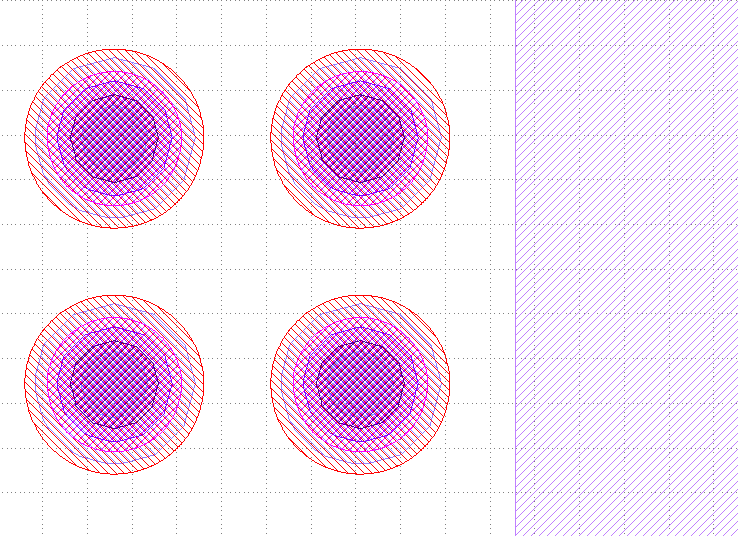
\includegraphics[width=0.8\textwidth]{figures/ActiveEdge/geometry_20NGR.png}};

      \begin{scope}[x={(image.south east)},y={(image.north west)}]

        \draw[blue, thick](0.62, 0.1)--(0. 62, 0.7);
        \draw[blue, thick, dashed](0.58, 0.1)--(0.58, 0.7);
        \draw[blue, thick, dashed](0.3, 0.1)--(0.3, 0.7);

        \draw[blue, thick, dashed](0.3, 0.1)--(0.62, 0.1);
        \draw[blue, thick, dashed](0.3, 0.7)--(0.62, 0.7);

        \node[below, color=blue] at (0.3, 0.1) {-0.055 mm};
        \node[below, color=blue] at (0.58, 0.1) {0 mm};

        \draw[<->, blue, thick](0.51, 0.4)--(0.62, 0.4);
        \node[right, color=blue] at (0.62, 0.4) {Edge distance};

      \end{scope}
    \end{tikzpicture}
    \caption{20-NGR-50}
    \label{fig:Layout20_NGR}
  \end{subfigure}~
  \begin{subfigure}[t]{0.5\textwidth}
    \centering
    \begin{tikzpicture}
      \node[anchor=south west,inner sep=0] at
      (0,0){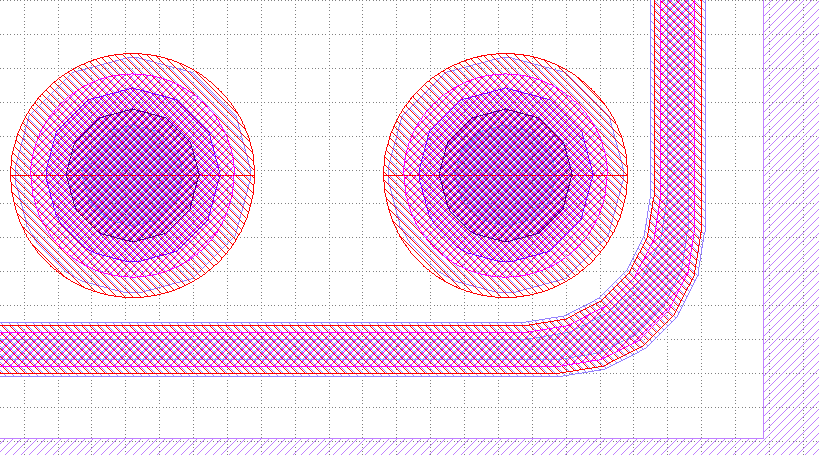
\includegraphics[width=0.8\textwidth]{figures/ActiveEdge/geometry_23FGR.png}};
    \end{tikzpicture}
    \caption{23-FGR-50}
    \label{fig:Layout20_FGR}
  \end{subfigure}
  \begin{subfigure}[t]{0.5\textwidth}
    \centering
    \begin{tikzpicture}
      \node[anchor=south west,inner sep=0] at
      (0,0){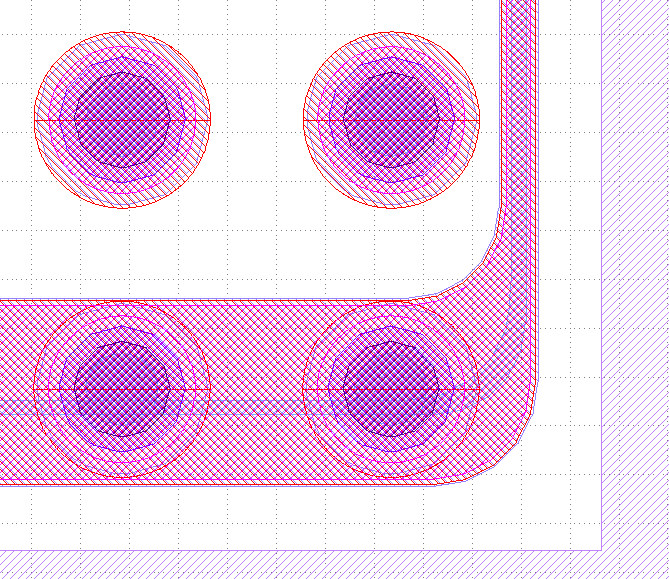
\includegraphics[width=0.55\textwidth]{figures/ActiveEdge/geometry_28GNDGR.png}};
    \end{tikzpicture}
    \caption{28-GNDGR-50}
    \label{fig:Layout20_GNDGR}
  \end{subfigure}~
  \begin{subfigure}[t]{0.5\textwidth}
    \centering
    \begin{tikzpicture}
      \node[anchor=south west,inner sep=0] at
      (0,0){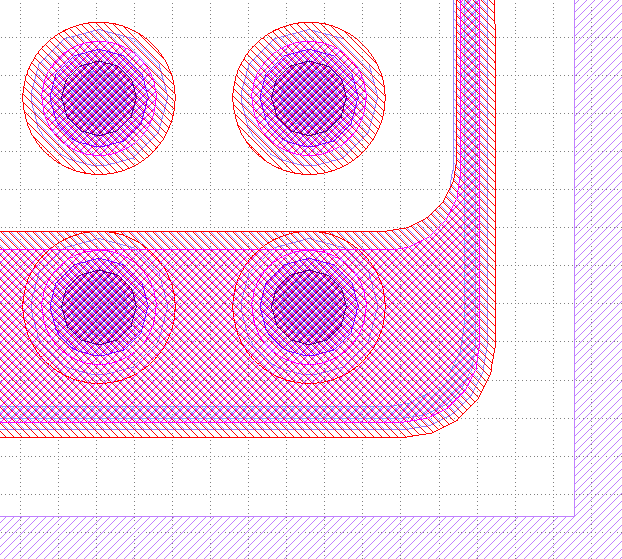
\includegraphics[width=0.55\textwidth]{{figures/ActiveEdge/geometry_55GNDGR.png}}};
    \end{tikzpicture}
    \caption{55-GNDGR-50, 55-GNDGR-100, 55-GNDGR-150}
    \label{fig:Layout50_GNDGR}
  \end{subfigure}~
  \caption{Sensor layouts for different guard-ring solutions for the
    assemblies described in \cref{tab:ActiveEdgeAssemblies}. (a) shows
    the convention used in the following sections to express the
    efficiency and the charge distribution at the edge as a function
    of the track position. The border of the last pixel before the
    edge is indicated by a dashed line (at position 0 mm) and the
    physical sensor edge with a continuous line.}
  \label{fig:Layout_guard_ring}
\end{figure}


\begin{figure}[htbp]
  \centering
  \begin{minipage}[t]{.4\textwidth}
    \centering
    \vspace{0pt}
    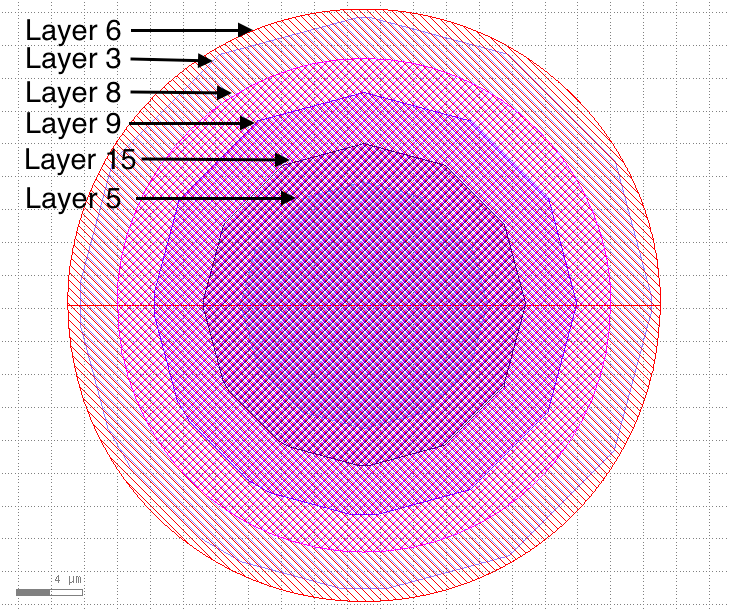
\includegraphics[width=0.95\textwidth]{figures/ActiveEdge/pixelLayout_withLayers.png}
    \caption{The different layers in the geometry description used for
      the sensor production.}
    \label{fig:PixelLayout}
  \end{minipage}
  \hfill
  \begin{minipage}[t]{.56\textwidth}
    \centering
    \vspace{0pt}
    \captionof{table}{Layers in the geometry description used for the
      sensor production (Picture from 23-FGR).}
    \label{tab:PixelStackDimensions}
    \begin{tabular}{l l}
      \toprule
      Layer number & Layer \\
      \midrule
      6 & metal\\
      3 & mask to etch oxide \\
      8 & pixel implant \\
      9 & UBM \\
      15 & passivation opening \\
      5 & contact to connect Al to Si \\
      \bottomrule
    \end{tabular}
  \end{minipage}
\end{figure}

\begin{table}
  \centering
  \captionof{table}{The dimensions of the different implants in for
    the sensors listed in \cref{tab:ActiveEdgeAssemblies}. The
    edge distance is the distance between the last pixel implant to
    the physical edge of the sensor as illustrated in
    \cref{fig:Layout20_NGR}. The metal width
    is the diameter of the metal layer for the pixels. The doping width is the
    diameter of the pixel implant. The contact width is the diameter of
    the contact between silicon and metal. The GR offset is the
    distance between the physical edge of the sensor and the implant
    of the guard ring. GR doping width, contact width and metal with
    are respectively the width of the implant, the contact and the
    metal layer for the guard ring.}
  \label{tab:DimensionsForAssemblies}
  \begin{tabular}{l c c c c}
    \toprule
    & 20-NGR-50 & 23-FGR-50 & 28-GNDGR-50 & 55-GNDGR-50, 100, 150 \\
    \midrule
    Edge width [\micron] & 20 & 23 & 28 & 55 \\
    Metal width [\micron] & 40 & 36 & 36 & 40 \\
    Doping width [\micron] & 30 & 30 & 30 & 30 \\
    Contact width [\micron] & 15 & 15 & 15 & 15 \\
    GR offset [\micron] & - & 10 & 14.5 & 25 \\
    GR doping width [\micron] & - & 5 & 5 & 5 \\
    GR contact width [\micron] & - & 3 & 3 & 3 \\
    GR metal width [\micron] & - & 7 & 7 & 10 \\
    \bottomrule
  \end{tabular}
\end{table}

%% --------------------------------------------- %%
\newpage
\subsection{Process flow for the simulation of the active-edge designs}
\label{sec:processFlowTCAD}

TCAD simulations (see \cref{sec:TCAD}) are used to simulate the
fabrication process and the device operation of active edge
sensors. The electric field and the electrostatic potential
distributions within the sensor are calculated. For realistic
simulations, the real dimensions of the assemblies as listed in
\cref{tab:DimensionsForAssemblies} are used. Due to the computational
power required for such simulations, the simulation is restricted to
two pixels in a 2D configuration as shown in \cref{fig:activeedge}.

The fabrication process of the sensors is simulated as follows:
\begin{enumerate}
\item The dimensions of the pixels, implants, contacts and metal
  layers are defined.
% \item The meshing is refined at the borders of the sensor and around the
%   implants based on the concentration of the dopants using an adaptive
%   meshing with the command \texttt{refinebox}.
\item The silicon region is then defined for two pixels, the edge
  region and an extra silicon edge which will be etched later (to make
  the process more realistic). From the bias scan, the depletion
  voltage is measured for the assemblies (see
  \cref{sec:ThinSensors_depletionVoltage}) and therefore the
  resistivity is adjusted accordingly to
  $\rho=10~\text{k}\Omega\text{cm}$.
  %The silicon is doped with borons (p-type material) with the initial resistivity of $\rho=10~\text{k}\Omega\text{cm}$ ($4.41\times 10^{11}\,\inversecmcubic$).
\item First a layer of $0.2\,\micron$ thick oxide and then a layer of
  $0.2\,\micron$ thick nitride are deposited on the top of the sensor.
\item The p-spray isolation technique is used to isolate the pixels
  from each other. Thus the silicon is implanted with borons at a
  concentration of $1\times10^{12}\,\inversecmsquared$. The
  implantation is done with an energy of $180\,\kev$.
\item The nitride is etched at the positions of the implants for the
  pixels and the guard ring if the assembly contains one. First a mask
  is put on the positions where the nitride is going to stay. Then the
  etching is done at the implantation positions. Phosphorus (n-type
  material) is implanted with a concentration of
  $1\times10^{15}\,\inversecmsquared$ with an energy of $120\,\kev$.

  % Masks limit the etching and the deposition to a certain
  % window and provide the possibility to imitate the lithographic
  % patterning.
\item The extra edge (as explained in point 2) is etched to achieve
  the edge distance of the assembly. In this process, first the
  nitride layer, then the oxide and finally the silicon layers are
  etched.
\item The sensor is flipped and a layer of oxide is deposited on the
  backside with a thickness of $0.04\,\micron$. Borons with a
  concentration of $1\times10^{15}\,\inversecmsquared$ and an energy
  of $60\,\kev$ are implanted. Then the oxide is etched from the
  backside and the sensor is flipped again to the initial position.
\item The oxide is etched at the contact positions.
\item The meshing of the edge is refined adaptively depending on the
  concentration of the ions and for a thickness of $1\,\micron$.
\item A photoresist is deposited on the top of the sensor with a
  thickness of $2\,\micron$.
\item Borons are implanted to the edge with a concentration of
  $1\times10^{15}\,\inversecmsquared$, an energy of $60\,\kev$ and a
  tilt of $15\degrees$.
\item The photoresist is removed.
\item To activate the dopants, the sensor is annealed at a constant
  temperature of $940\degrees$C during 240 minutes.
\item The pixels and guard ring metal layer is deposited using an
  aluminium layer with a thickness of $0.8\,\micron$.
\item A layer of aluminium with a thickness of $0.8\,\micron$ is
  deposited for the contact of the high-voltage on the back-side of
  the sensor.
\end{enumerate}
 

The resulting doping concentration for the different layouts is shown
in Figure~\ref{fig:TCAD_dopingConcentration}.

%% --------------------------------------------- %%
\newpage
\section{Electrical measurements and simulations}

In silicon, the breakdown occurs for electric fields exceeding
$\sim3\times10^5$~\voltpercm~\cite{Sze:100213}. In active-edge
sensors, since the back-side implantation as well as the bias voltage
are extended to the edge of the sensor, the gradient of potential
between the edge and the last pixel can be very high. This could lead
to a breakdown of the sensor.

\cref{fig:IVmeasurements_real} shows the measured leakage current in
the different assemblies as a function of the bias voltage. For the
nominal operation (at -15~V for $50\,\micron$, -20~V for
$100\,\micron$ and -30~V for $150\,\micron$ thick sensors), none of
the assemblies are operated beyond the breakdown voltage. The
breakdown occurs earlier for the assembly without guard ring
(20-NGR-50) compared to the other assemblies. The $50\,\micron$ thick
assemblies with the floating guard ring (23-FGR-50) and the grounded
guard ring (28-GNDGR-50 and 55-GNDGR-50) lead to a similar
breakdown. However, the floating guard ring is expected to smoothen
the potential transition between the edge of the sensor and the first
pixel and result in a later breakdown voltage. This can be explained
by the fact that the Timepix3 chip provides an extra row of pixels
giving the possibility to connect the guard ring to the ground
potential. The edge of 23-FGR-50 might get too close to the extra row
of pixels leading to a high potential gradient in that region. The
thicker sensors show a later breakdown.

% This could be explained by the fact that Timepix3 provides an
% extra row of pixels giving the possibility to connect the guard ring
% to the ground potential. The floating guard ring may touch this extra
% row and this makes a floating guard ring similar to a grounded one in
% terms of leakage current. 

\begin{figure}[htbp]
  \centering
  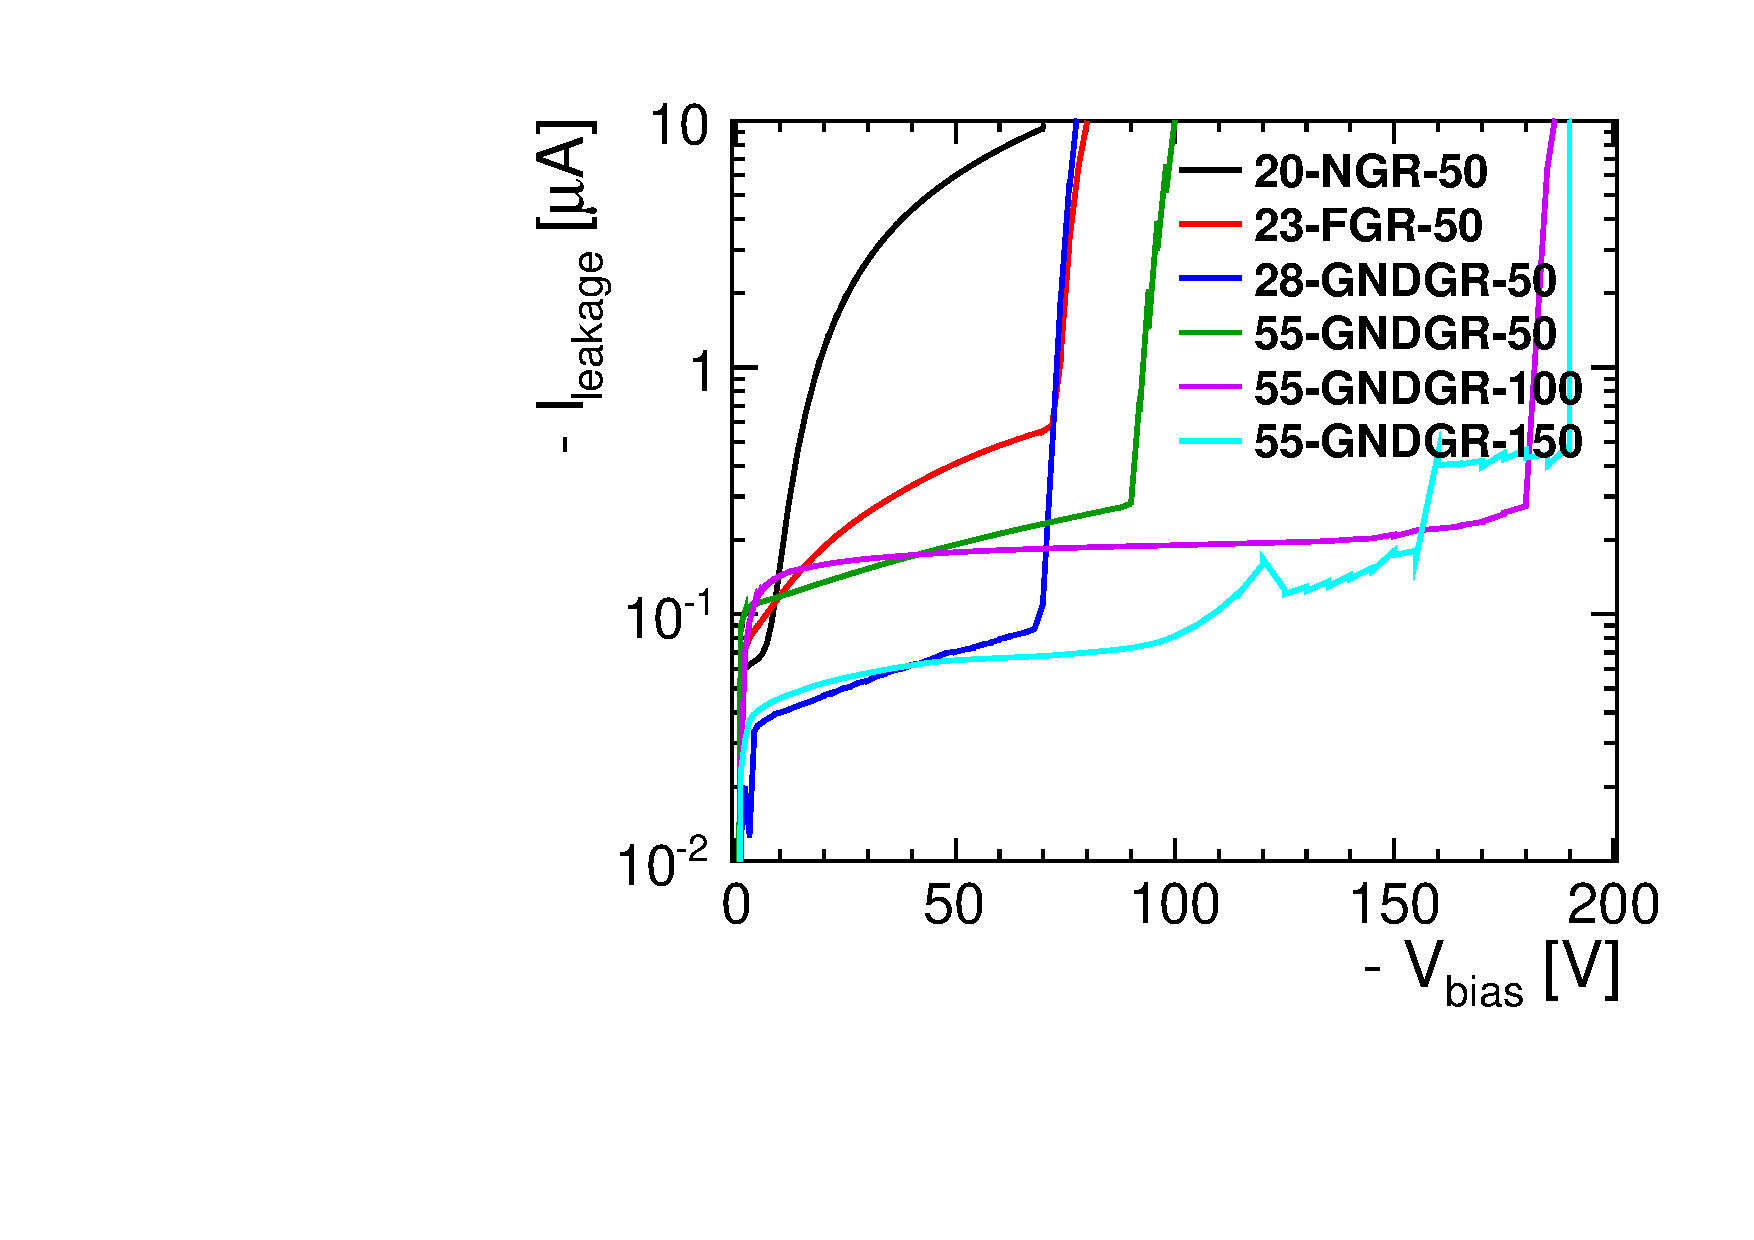
\includegraphics[width=0.6\textwidth]{figures/ActiveEdge/IVCurve_Andreas.pdf}
  \caption{Measured leakage current for active-edge assemblies listed
    in \cref{tab:ActiveEdgeAssemblies}. For all assemblies, the
    measurements were done at the room temperature of $22^{\circ}$~C.}
  \label{fig:IVmeasurements_real}
\end{figure}




In TCAD simulations, the electric field distribution for the sensors
operated at nominal conditions are shown in
\cref{fig:TCAD_Efield2D}. In all cases, for the nominal conditions
(see \cref{tab:nominalBiasThreshold}), the breakdown electric field is
not reached in agreement with the simulated currents (see
\cref{fig:IVmeasurements_TCAD}).

\begin{figure}[htbp]
  \centering
  \begin{subfigure}[b]{0.5\textwidth}
    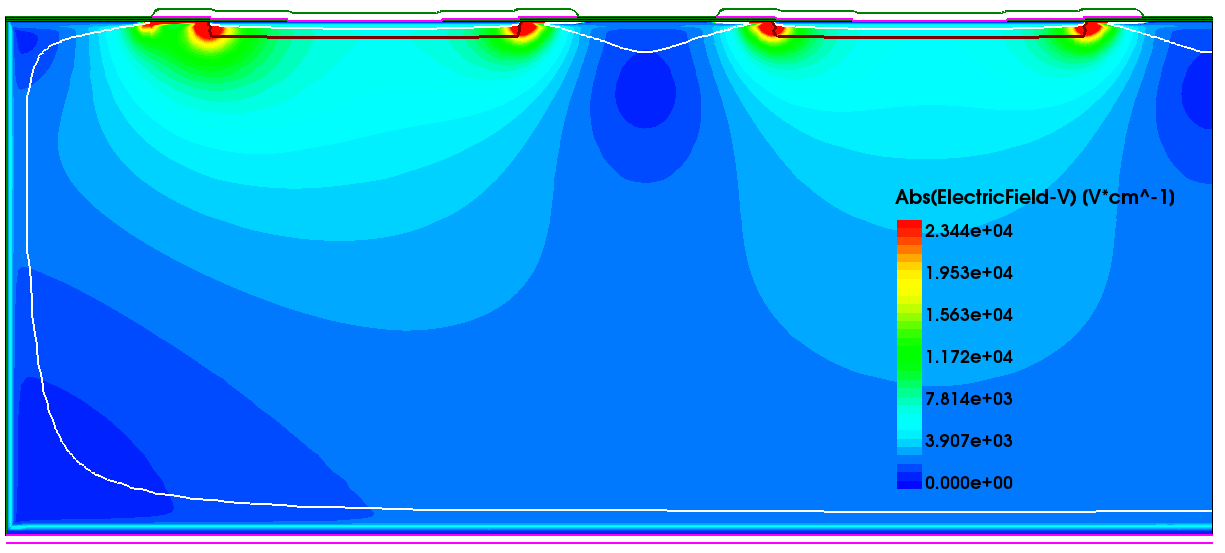
\includegraphics[width=\textwidth]{figures/ActiveEdge/Efield_20_NGR.png}
    \caption{20-NGR-50}
  \end{subfigure}\hfill
  \begin{subfigure}[b]{0.5\textwidth}
    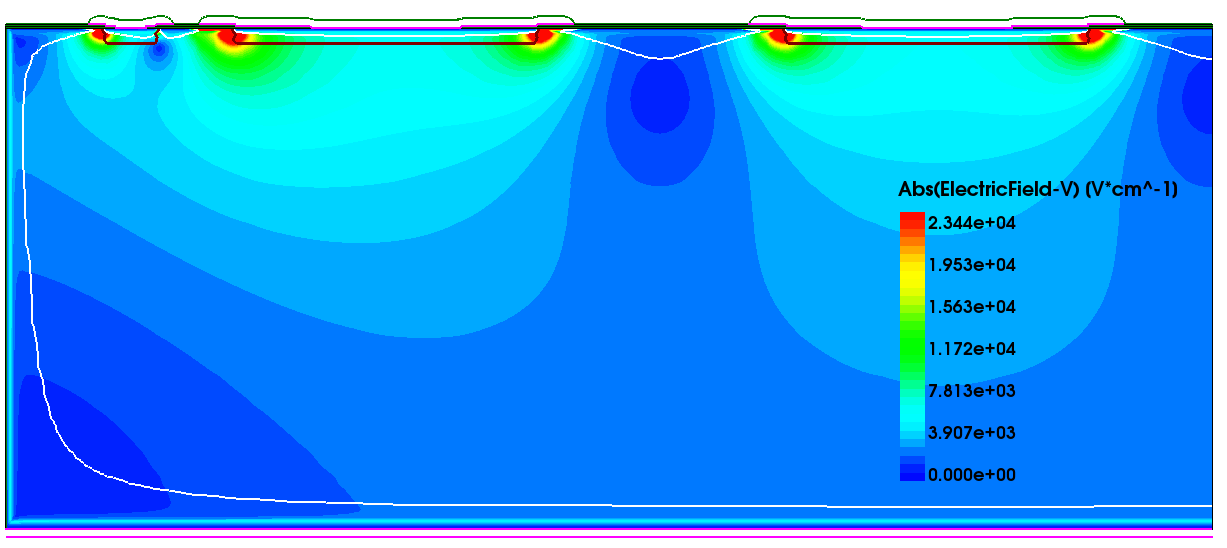
\includegraphics[width=\textwidth]{figures/ActiveEdge/Efield_23_FGR.png}
    \caption{23-FGR-50}
  \end{subfigure} \\
  \begin{subfigure}[b]{0.5\textwidth}
    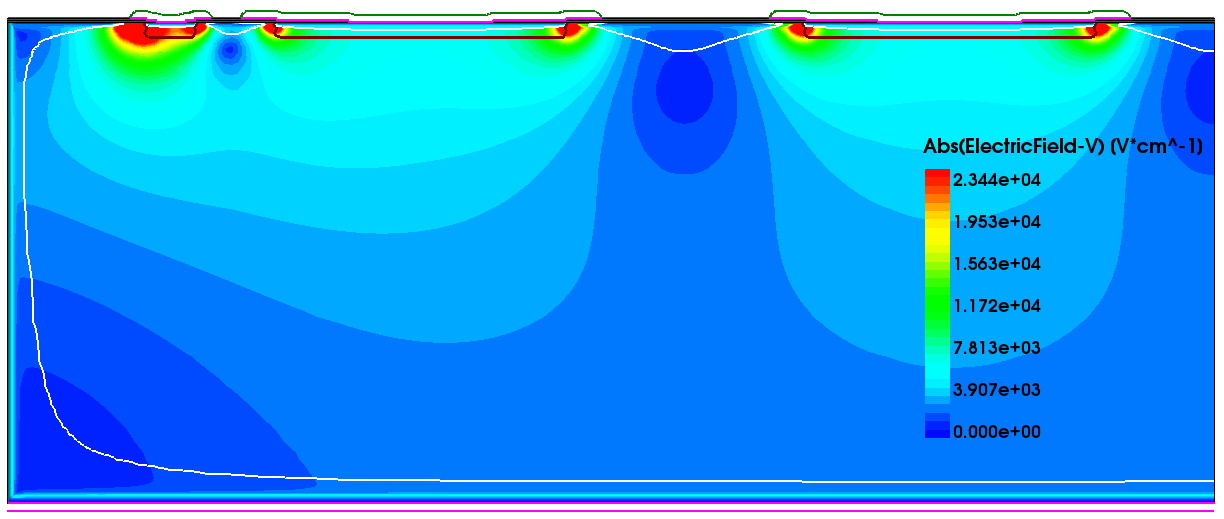
\includegraphics[width=\textwidth]{figures/ActiveEdge/Efield_28_GNDGR.png}
    \caption{28-GNDGR-50}
  \end{subfigure}\hfill
  \begin{subfigure}[b]{0.5\textwidth}
    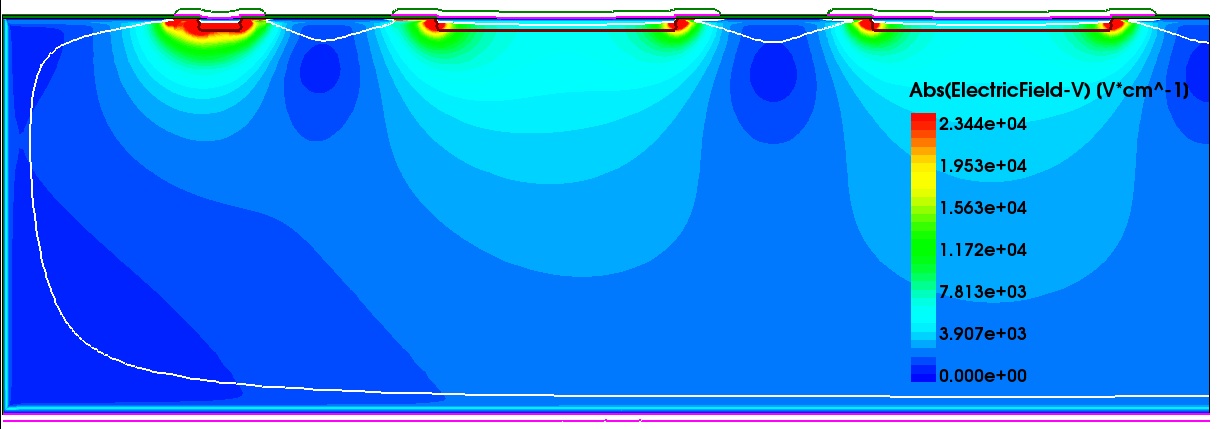
\includegraphics[width=\textwidth]{figures/ActiveEdge/Efield_55_GNDGR.png}
    \caption{55-GNDGR-50}
  \end{subfigure} \\
  \begin{subfigure}[b]{0.5\textwidth}
    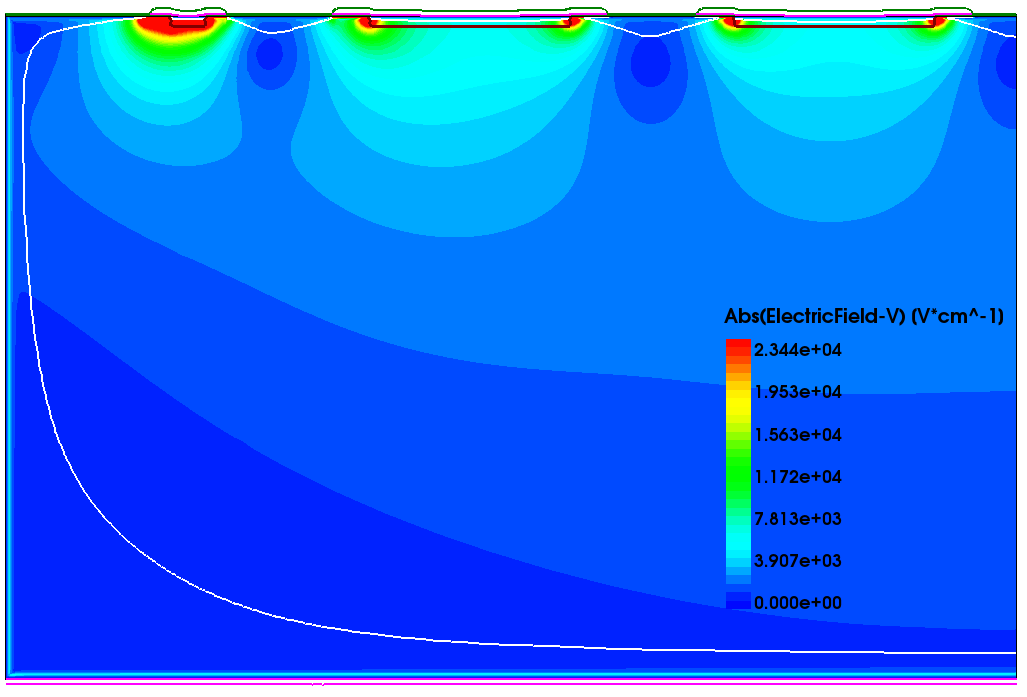
\includegraphics[width=\textwidth]{figures/ActiveEdge/Efield_55_GNDGR_100.png}
    \caption{55-GNDGR-100}
  \end{subfigure}\hfill
  \begin{subfigure}[b]{0.5\textwidth}
    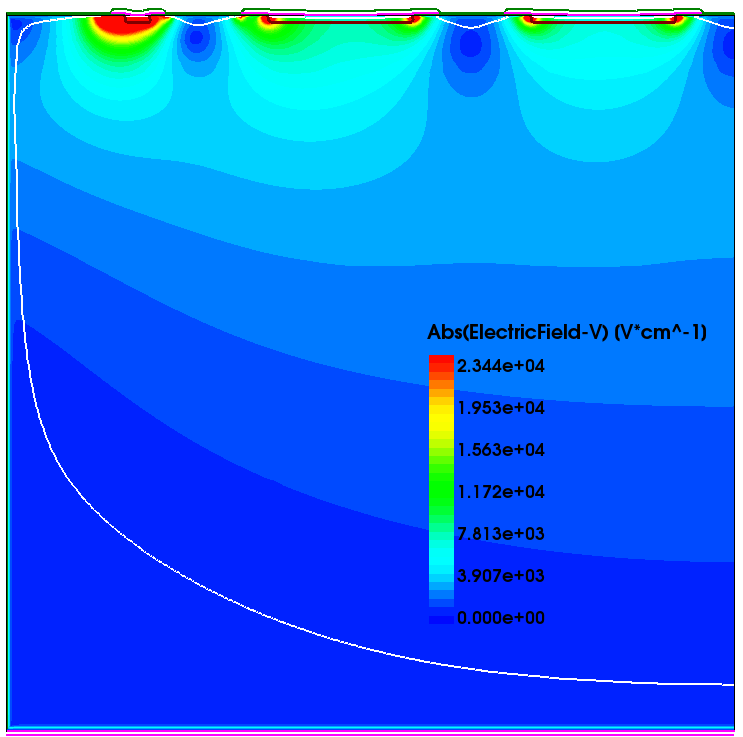
\includegraphics[width=\textwidth]{figures/ActiveEdge/Efield_55_GNDGR_150.png}
    \caption{55-GNDGR-150}
  \end{subfigure}
  \caption{Electric field distribution in TCAD simulations for the
    assemblies listed in \cref{tab:ActiveEdgeAssemblies}. The
    depletion region is shown with the white line.}
  \label{fig:TCAD_Efield2D}
\end{figure}


The electric field and the electrostatic potential in TCAD simulations
for a cut close to the n-implants ($0.2\,\micron$ from the sensor
surface) are shown in
\cref{fig:TCAD_Efield_EPotential_sensorSurface}. Position $0\,\micron$
corresponds to the position of the first pixel. The floating
guard-ring (23-FGR-50) results in a smoother potential transition
between the edge of the sensor and the first pixel.


\begin{figure}[htbp]
  \centering
  \begin{subfigure}[b]{0.5\textwidth}
    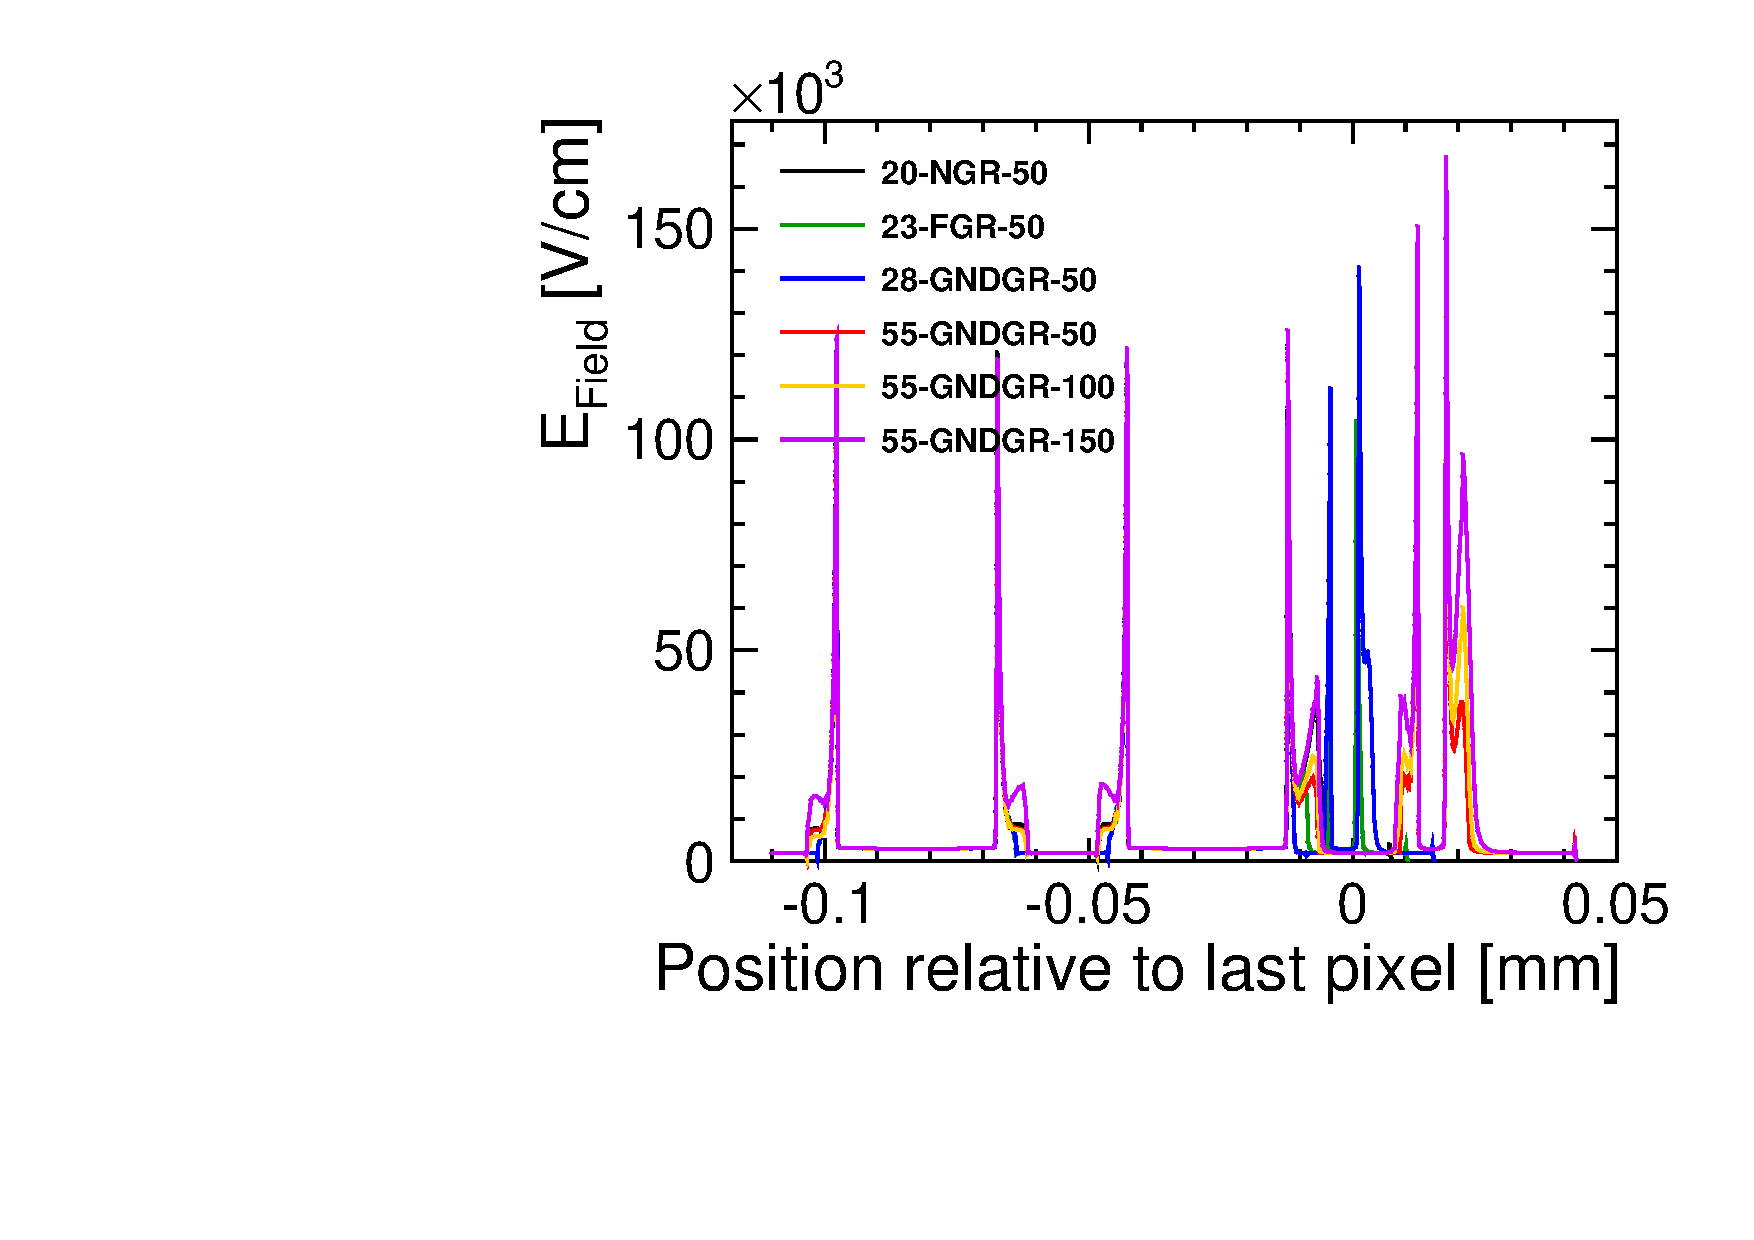
\includegraphics[width=\textwidth]{figures/ActiveEdge/Efiel_cut0_2um.pdf}
    \caption{}
  \end{subfigure}\hfill
  \begin{subfigure}[b]{0.5\textwidth}
    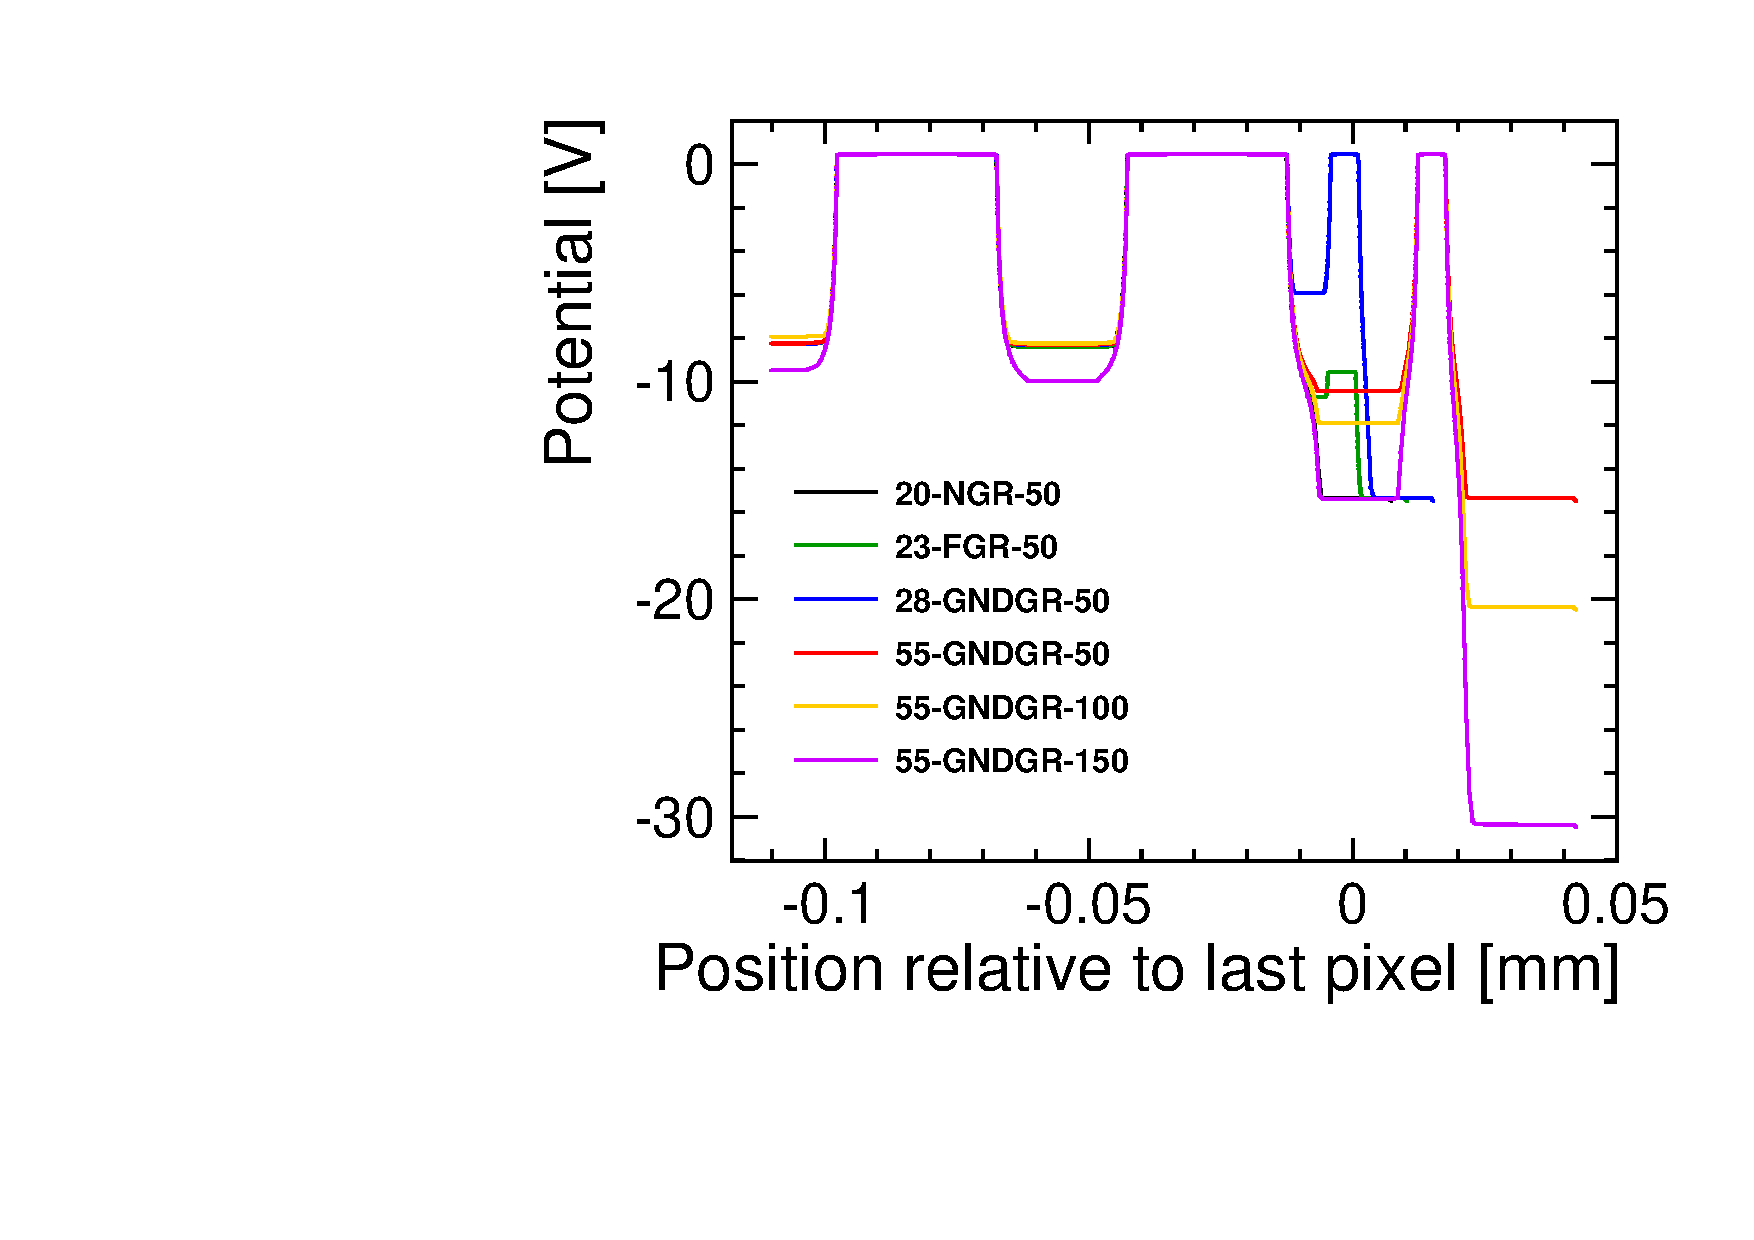
\includegraphics[width=\textwidth]{figures/ActiveEdge/EPotential_cut0_2um.pdf}
    \caption{}
  \end{subfigure}
  \caption{(a) The electric field and (b) the electrostatic potential
    for nominal bias voltage at a distance of $0.2\,\micron$ below the
    sensor surface. Position $0\,\micron$ corresponds to the position
    of the first pixel.}
  \label{fig:TCAD_Efield_EPotential_sensorSurface}
\end{figure}


\cref{fig:IVmeasurements_TCAD} shows the leakage current obtained from
the TCAD simulations for the simulated pixel cell. In TCAD
simulations, only the sensor is simulated and the effect of the
readout chip and the bump bonding are not included. The readout chip
can increase the temperature and increase the leakage current. 

In simulations, the assemblies with grounded guard ring (including all
sensor thicknesses) and without guard ring show a breakdown of the
junction at around 150~V. In these sensors, the distance between the
edge implant (with high voltage) and the ground implant (either the
pixel or the guard ring) is similar which leads to a similar potential
gradient and breakdown voltage. As expected, the floating guard ring
shows a higher breakdown voltage of 240~V.

%% The current calculated from the 2D simulation is scaled to obtain the
%% current in the total matrix.

\begin{figure}[htbp]
  \centering
  \begin{subfigure}[b]{0.45\textwidth}
    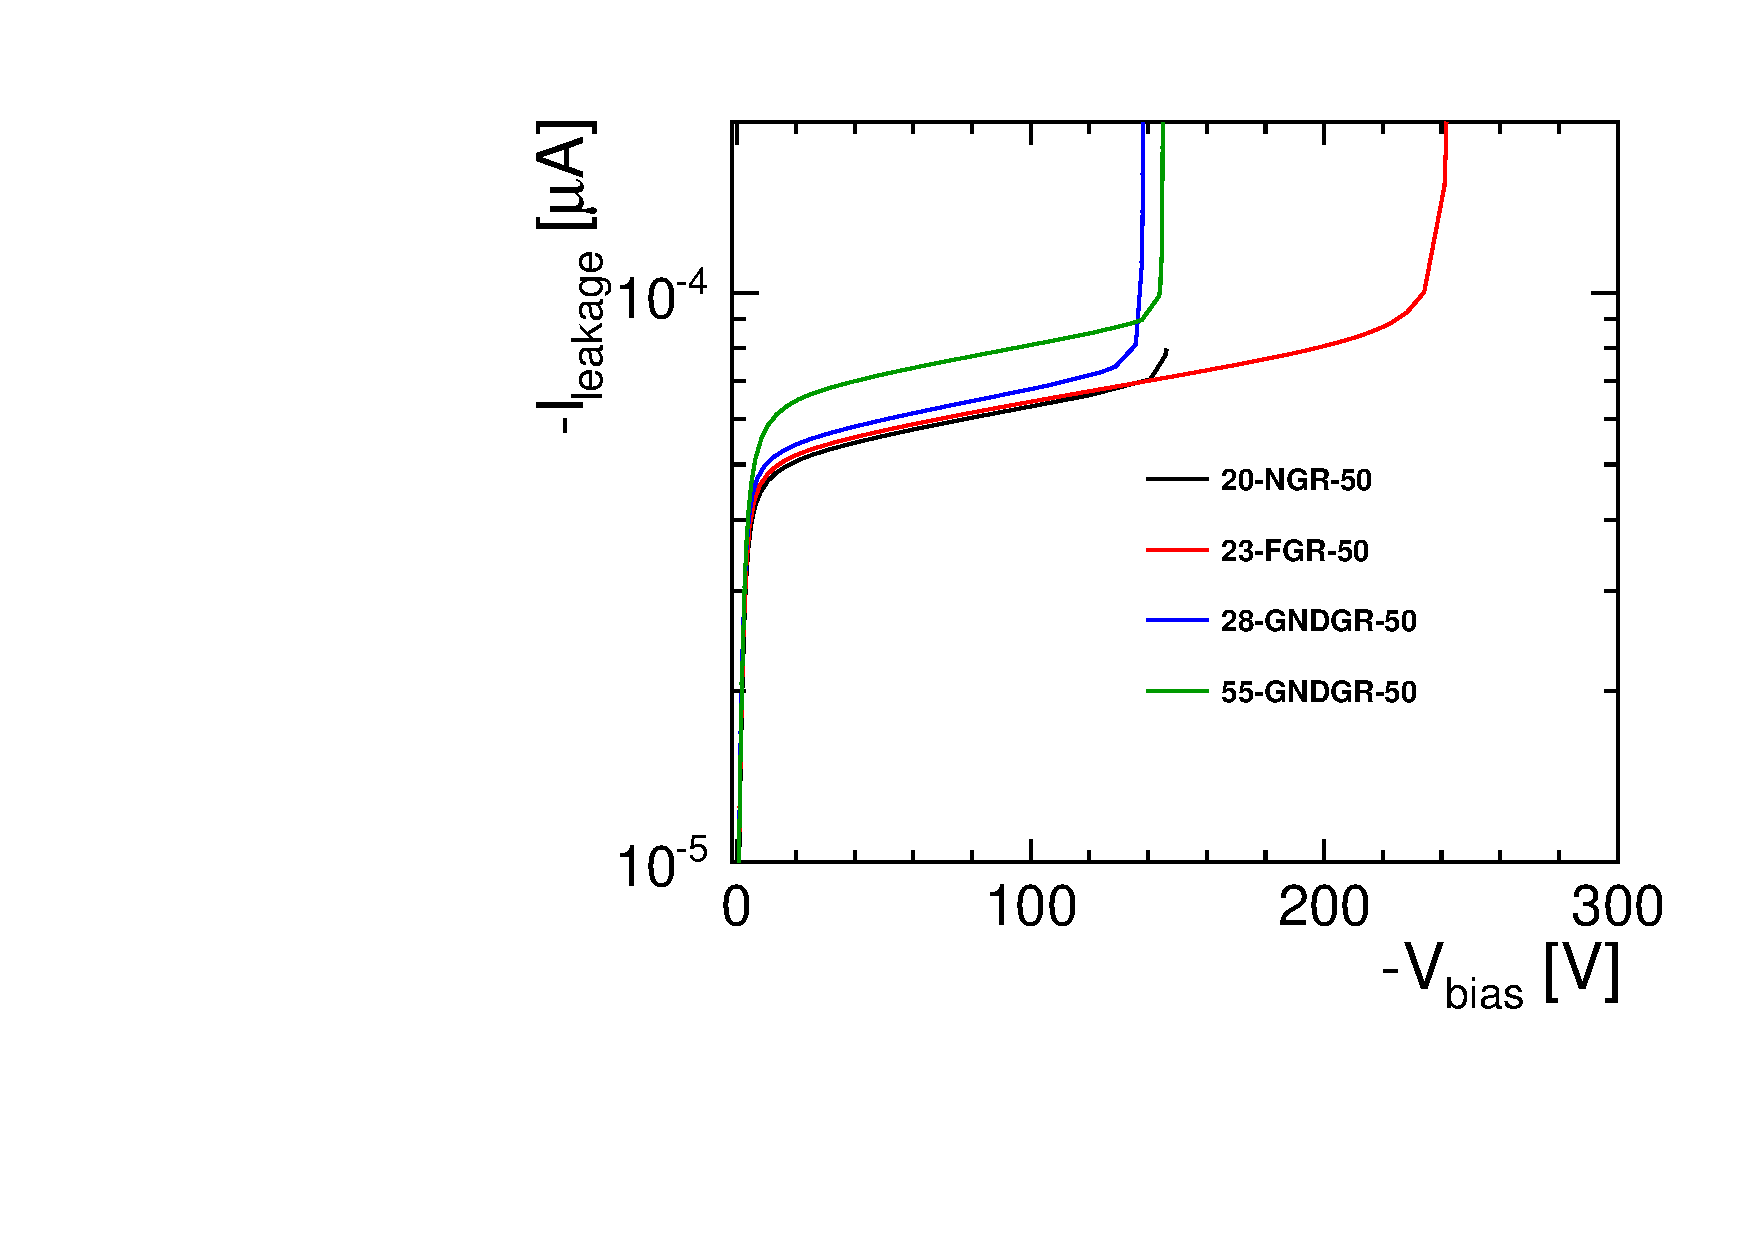
\includegraphics[width=\textwidth]{figures/ActiveEdge/IVCurve_TCAD_50_micron.pdf}
    \caption{}
  \end{subfigure}\hfill
  \begin{subfigure}[b]{0.45\textwidth}
    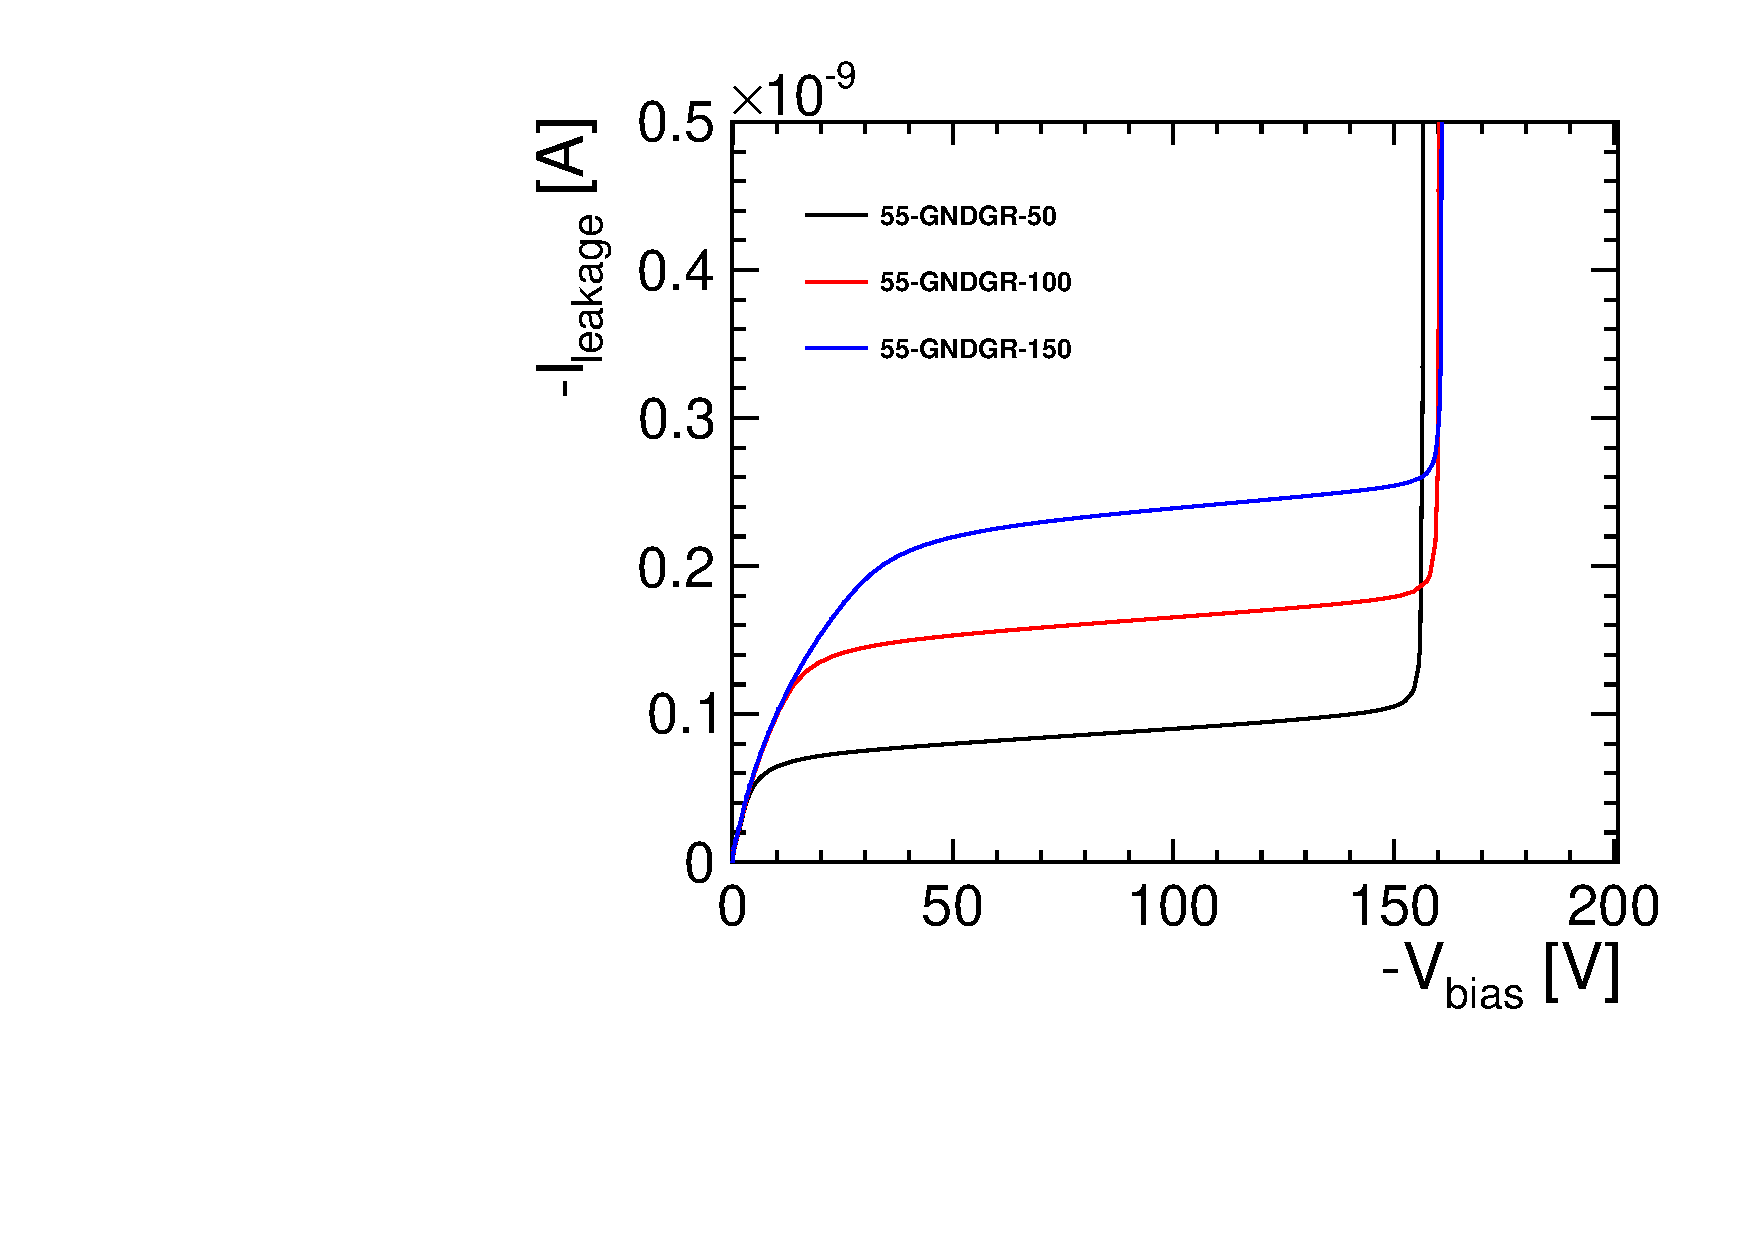
\includegraphics[width=\textwidth]{figures/ActiveEdge/IVCurve_TCAD_55_GNDGR.pdf}
    \caption{}
  \end{subfigure}
  \caption{Leakage current in TCAD simulations for the pixel cell as a
    function of bias voltage for (a) $50\,\micron$ thick sensors and
    for (b) assemblies with a grounded guard ring (refer to
    \cref{tab:ActiveEdgeAssemblies} for the details on the assemblies).}
  \label{fig:IVmeasurements_TCAD}
\end{figure}

%% --------------------------------------------- %%
\newpage
\section{Edge performance in data and simulations}
The active-edge assemblies are tested at the CERN SPS with $120\,\gev$
pions (see \cref{sec:CERN_SPS}), making use of the CLICdp Timepix3
beam reference telescope as described in \cref{ch:Telescope}. The
collected charge at the edge is also simulated (as described in
\cref{sec:TCAD_Simu_ActiveEdge}) and compared to the data. The edge
performance is investigated in terms of the efficiency of detecting a
track and the amount of collected charge as a function of the track
position at the edge.

%% --------------------------------------------- %%
\subsection{TCAD simulation of the detector response}
\label{sec:TCAD_Simu_ActiveEdge}

TCAD simulations are used to study the charge collection at the edge
region. The process flow as described in \cref{sec:processFlowTCAD} is
used to simulate two pixels and the edge region in a 2D
configuration. The transient simulation of the active edge devices is
done by a constant charge deposition corresponding to the peak of the
straggling function along the particle track (see
\cref{sec:SiliconEnergyLossSpectrum}). \cref{fig:TCAD_transientSimu}
illustrates an example of a MIP traversing the sensor at a distance of
$10\,\micron$ from the left edge. The electron density 1~ns after the
particle hits the sensor is shown.



\begin{figure}[htbp]
  \centering
  \begin{tikzpicture}
    \node[anchor=south west,inner sep=0] (image) at
    (0,0){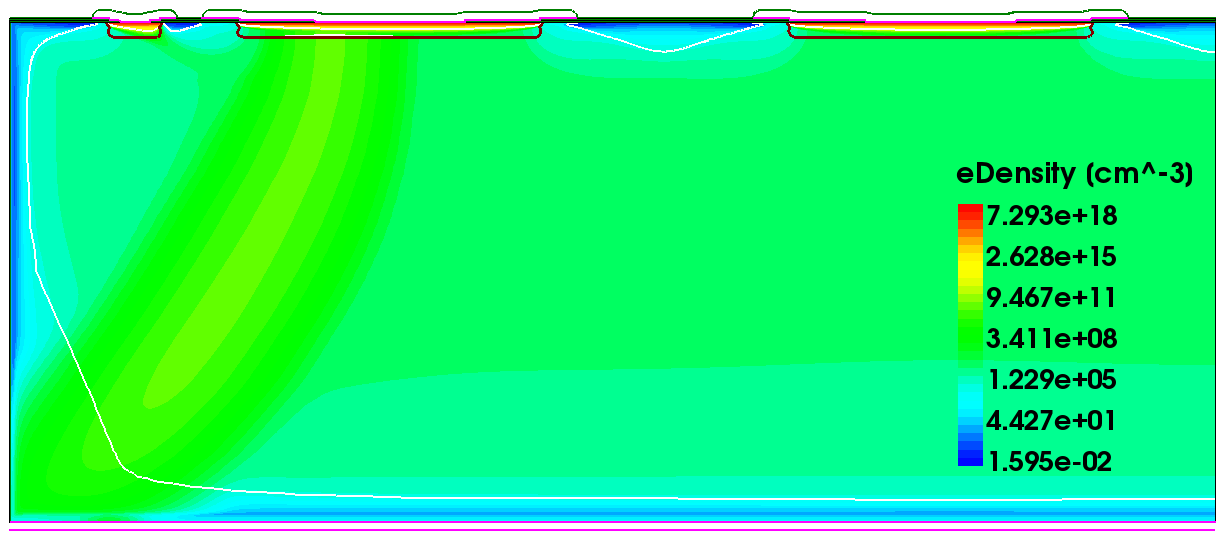
\includegraphics[width=0.7\textwidth]{figures/ActiveEdge/TCAD_transient_23FGR_hitpos_60.png}};
    \begin{scope}[x={(image.south east)},y={(image.north west)}]

      %% \draw[help lines,xstep=.1,ystep=.1] (0, 0) grid (1,1);
      %% \foreach \x in {0,1,...,9} { \node [anchor=north] at (\x/10,0) {0.\x}; }
      %% \foreach \y in {0,1,...,9} { \node [anchor=east] at (0,\y/10) {0.\y}; }

      \draw[->, very thick] (0.093, 0.0) -- (0.093, 1.05);
    \end{scope}
  \end{tikzpicture}
  \caption{Transient simulation of a particle track traversing the
    sensor with a floating guard ring at a distance of $10\,\micron$
    from the edge (illustrated as an arrow). The electron density 1~ns
    after the particle hit is shown. The region shown with a white
    line is the depletion region.}
  \label{fig:TCAD_transientSimu}
\end{figure}

In simulation, hits are generated at different positions along the
edge. The electrodes collect the signal pulse and integrate it over
15~ns. The peaking time of the signal is usually less than 5~ns
therefore the integration time is enough to collect most of the
signal.



%% --------------------------------------------- %%
\subsection{Conventions used for the presentation of the results}
\label{sec:activeEdge_convention}

The convention as illustrated in \cref{fig:Layout20_NGR} is used to
show the performance of the different assemblies in
\cref{sec:EdgePerformance_50,sec:EdgePerformance_100_150}. The border
of the last pixel (at 0~mm) is indicated with a dashed line and the
physical sensor edge is shown as a continuous line. The detection
efficiency is calculated by counting the number of tracks matched to
hits on the DUT (with a distance criterion of $100\,\micron$) divided
by the total number of tracks projected on the DUT. The efficiency
within the pixels is then mapped into a grid of $2\times2$ pixels. The
x-axis shows the track position relative to the last pixel. The y-axis
combines the tracks for the even rows (in the coordinates between 0~mm
and 0.055~mm) and the odd rows (in the coordinates between 0.055~mm
and 0.11~mm). The z-axis shows the efficiency. To increase the number
of tracks close to the sensor edge, the beam was focused on only one
of the edges during the data taking. An example of the track impact
points for the assembly 20-NGR-50 is shown in \cref{fig:hitMapW19G7}.

\begin{figure}[htbp]
  \centering
  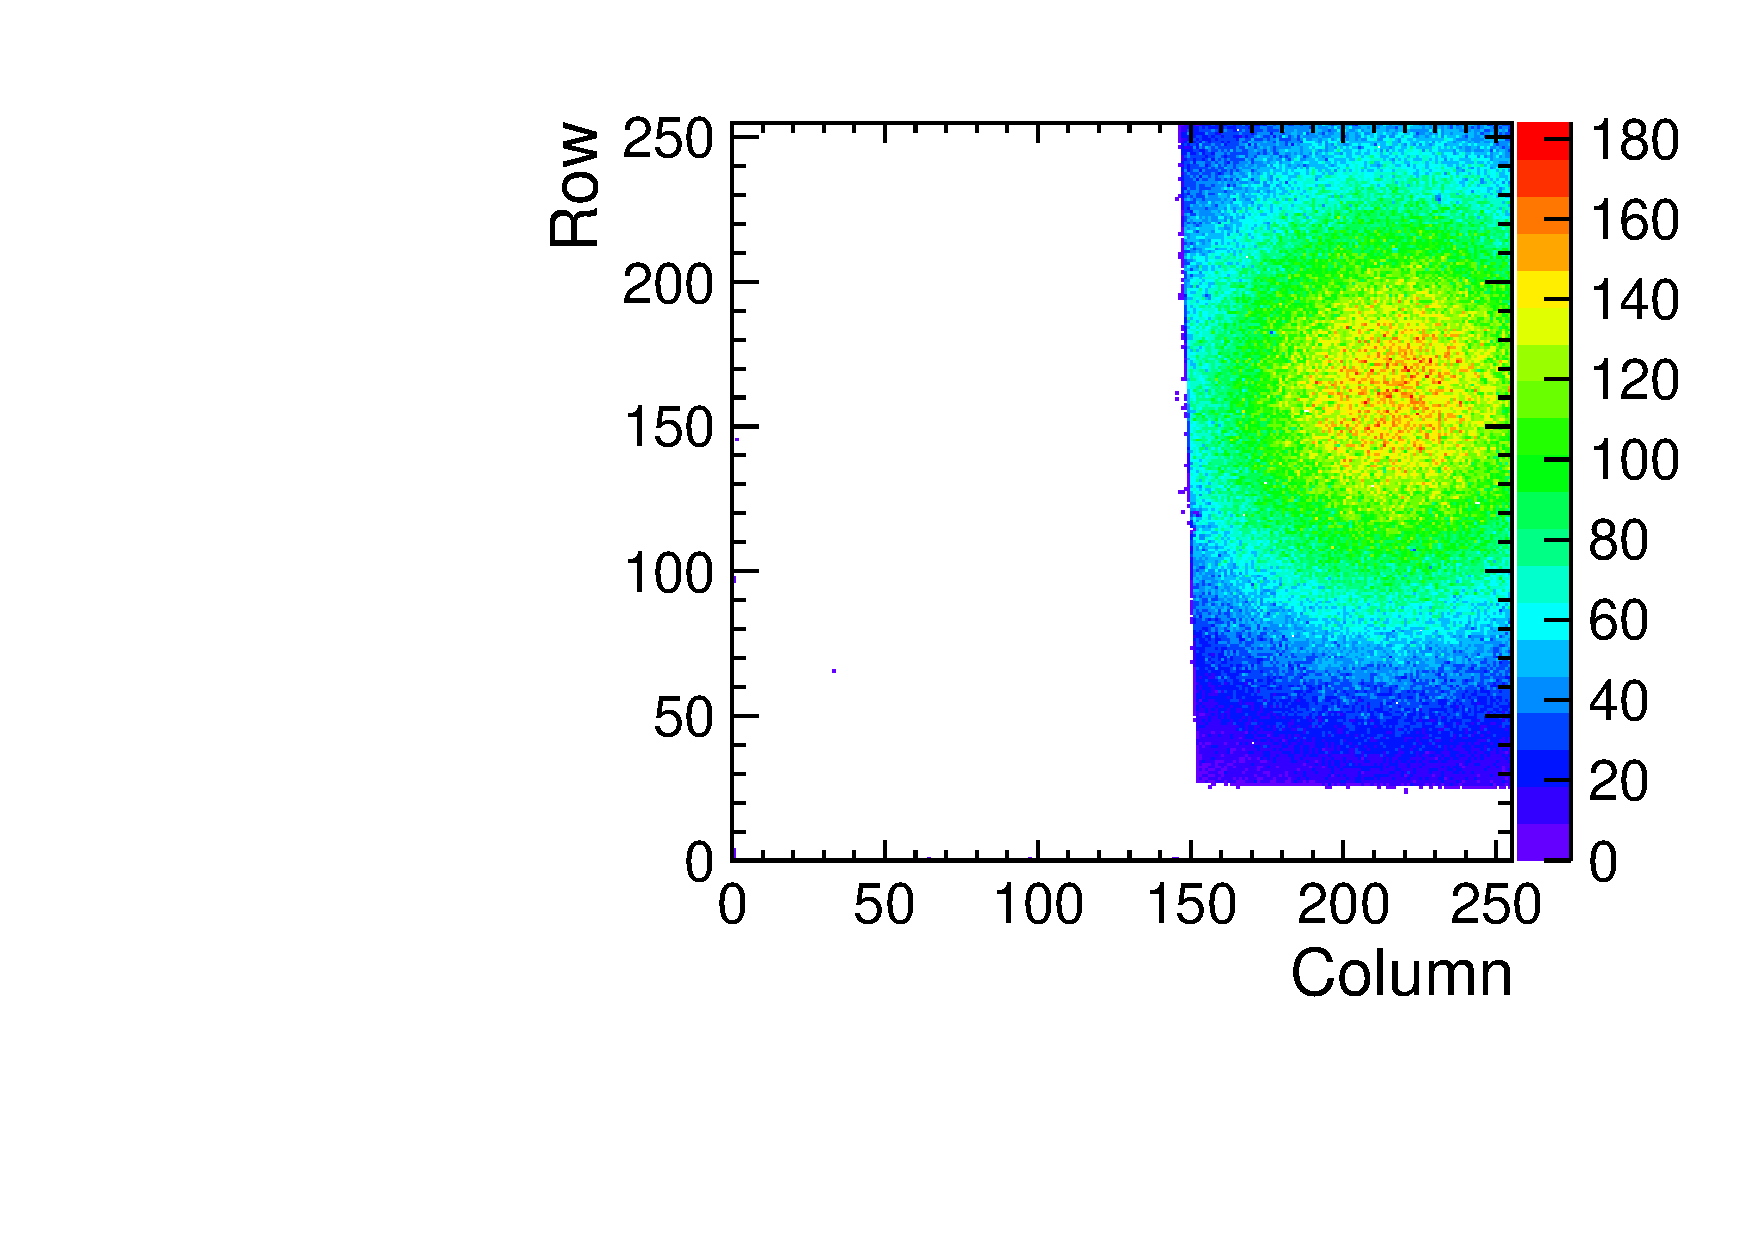
\includegraphics[width=0.7\textwidth]{figures/ActiveEdge/hitMap_W19_G7.pdf}
  \caption{The track impact points on the assembly 20-NGR-50: the beam
    is focused on the edge of the assembly in order to increase the
    statistics for the edge performance studies.}
  \label{fig:hitMapW19G7}
\end{figure}


The collected charge as a function of the track position is compared
in data and TCAD simulations. In data, the deposited charge is plotted
versus the track position given by the Timepix3 telescope (with a
resolution of $\sim2\,\micron$). The deposited charge is obtained by
applying the test-pulse calibrations to the TOT values measured in
data (see \cref{sec:EnergyCalibration}). The most-probable-value (MPV)
of the charge deposition in data is compared to the TCAD simulations.

To obtain the MPV of the energy deposition in data, only tracks within
the central $40\%$ of the pixel cell area are considered for all
assemblies except for 28-GNDGR-50 where only the central $7\%$ of the
pixel is considered. This reduces the influence of the regions between
the pixel implants in the row direction, which are not modeled in the
2D simulation. In these regions a larger loss of charge to the guard
ring is expected. To calculate the MPV in data, the distribution of
the deposited charge for each position is fitted with a Landau
function convoluted with a Gaussian. The most probable value (MPV) of
the Landau fit is then compared to the collected charge obtained in
the TCAD simulations. In the TCAD simulations, a fixed amount of
charge is deposited and the fluctuations of the deposited charge are
not considered.

The tracking resolution of $\sim2\,\micron$ is applied to the hit
position in TCAD simulations. This is done by convoluting a Gaussian
function with a standard deviation of $2\,\micron$ with the simulated
hit position. The border of the last pixel (at 0~mm) is indicated with
a dashed line and the physical sensor edge is shown as a continuous
line with the convention as illustrated in \cref{fig:Layout20_NGR}.

% This can explain the minor discrepancies on the
% amount of the collected charge between simulation and data. 

% The collected charge at the edge as a function of the track position
% is also investigated. The pixel-by-pixel calibration as described in
% \cref{sec:EnergyCalibration} is applied to convert the TOT value into
% the energy deposition in units of the number of collected electrons.

%% --------------------------------------------- %%
\subsection{The performance of $50\,\micron$ thick sensors}
\label{sec:EdgePerformance_50}

Exploiting the high tracking capabilities of the Timepix3 telescope,
the efficiency at the edge of the assemblies with $50\,\micron$ thick
sensors is shown in two dimensions in
\cref{fig:EdgeEfficiency_50micron}. The results are presented using
the conventions as described in \cref{sec:activeEdge_convention}.

\begin{figure}[htbp]
  \begin{subfigure}[b]{0.24\textwidth}
    \centering
    \includegraphics[width=\textwidth, page=3]{figures/TestBeam/edge_bcp.pdf}
  \caption{20-NGR-50}\label{fig:EdgeEfficiency_20NGR50}
  \end{subfigure}\hfill
  \begin{subfigure}[b]{0.24\textwidth}
    \centering
    \includegraphics[width=\textwidth, page=6]{figures/TestBeam/edge_bcp.pdf}
  \caption{23-FGR-50}\label{fig:EdgeEfficiency_23FGR50}
  \end{subfigure}\hfill
  \begin{subfigure}[b]{0.24\textwidth}
    \centering
    \includegraphics[width=\textwidth, page=9]{figures/TestBeam/edge_bcp.pdf}
  \caption{28-GNDGR-50}\label{fig:EdgeEfficiency_28GNDGR50}
  \end{subfigure}\hfill
  \begin{subfigure}[b]{0.24\textwidth}
    \centering
    \includegraphics[width=\textwidth, page=12]{figures/TestBeam/edge_bcp.pdf}
  \caption{55-GNDGR-50}\label{fig:EdgeEfficiency_55GNDGR50}
  \end{subfigure}
  \caption{The efficiency at the edge as a function of the track
    positions for the assemblies having a sensor thickness of
    $50\,\micron$.}
  \label{fig:EdgeEfficiency_50micron}
\end{figure}

The assemblies without (20-NGR-50) and with floating guard ring
(23-FGR-50) are efficient up to the physical edge of the sensor as
shown in
\cref{fig:EdgeEfficiency_20NGR50,fig:EdgeEfficiency_23FGR50}. \cref{fig:ChargeCollectionNGRFGR}
shows the charge collected at the edge as a function of the track
position in data and TCAD simulations for 20-NGR-50 and 23-FGR-50. The
charge is fully collected by the last pixel for 20-NGR-50. For
23-FGR-50, a loss of the charge near the edge is observed.

For 20-NGR-50, the TCAD simulation agrees well with the data
observation as shown in \cref{fig:ChargeCollection20NGR}.

To simulate a floating guard ring for 23-FGR-50 in TCAD, the current
on the electrode of the guard ring is set to zero. The charge drop in
the edge is explained by the capacitive coupling between the guard
ring and the surrounding implants. Data shows a higher charge drop in
the edge than the TCAD simulations. This is expected, as the 2D
simulation does not include the capacitive coupling over the full
length of the guard ring.

% To have a more accurate definition
% of the capacitive coupling in TCAD simulations, for this guard ring
% configuration, the area factor is set to the pixel size in order to
% multiply the currents in the electrodes by this factor. This defines
% the third dimension in a 2D simulation.

\begin{figure}[htbp]
  \begin{subfigure}[b]{0.45\textwidth}
    \centering
    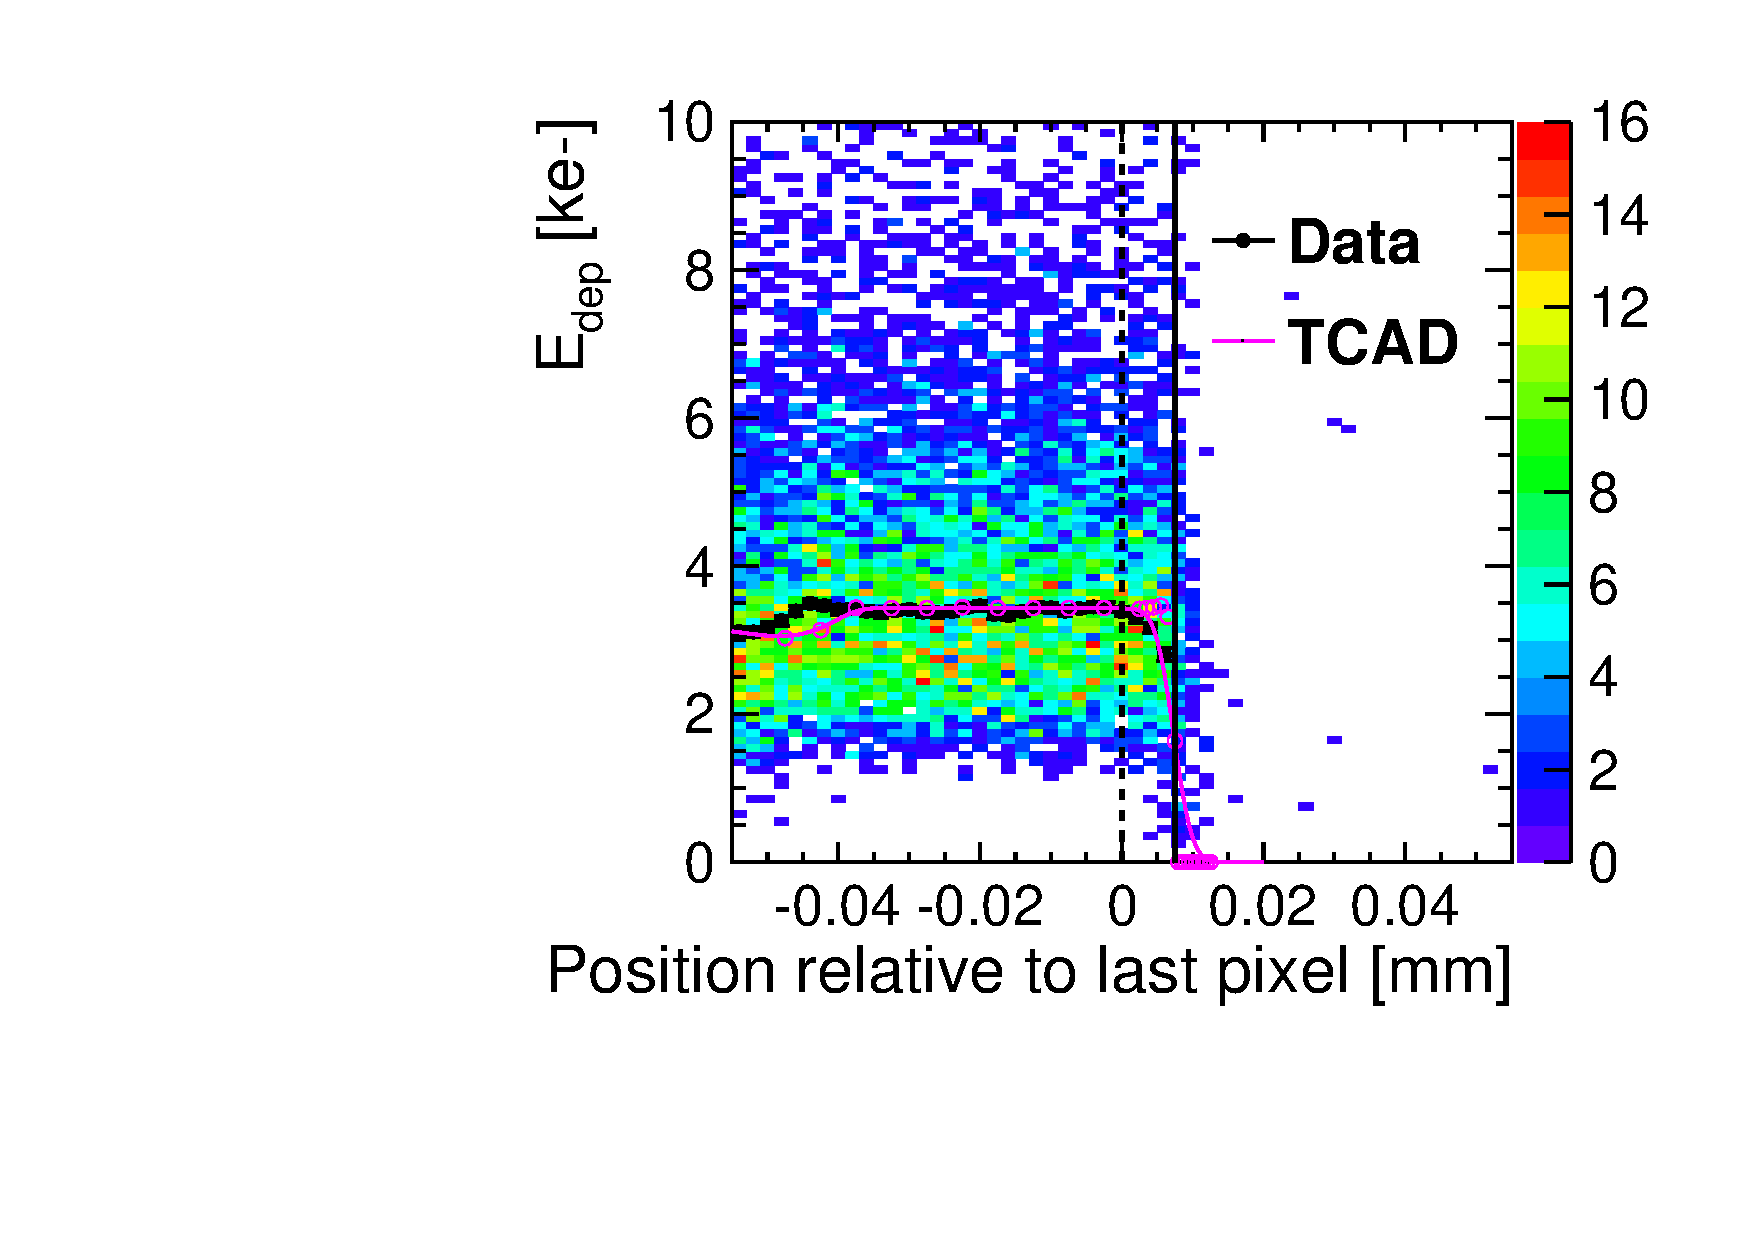
\includegraphics[width=\textwidth]{figures/ActiveEdge/20_NGR_Edep_TCAD_data.pdf}
    \caption{20-NGR-50}\label{fig:ChargeCollection20NGR}
  \end{subfigure}\hfill
  \begin{subfigure}[b]{0.45\textwidth}
    \centering
    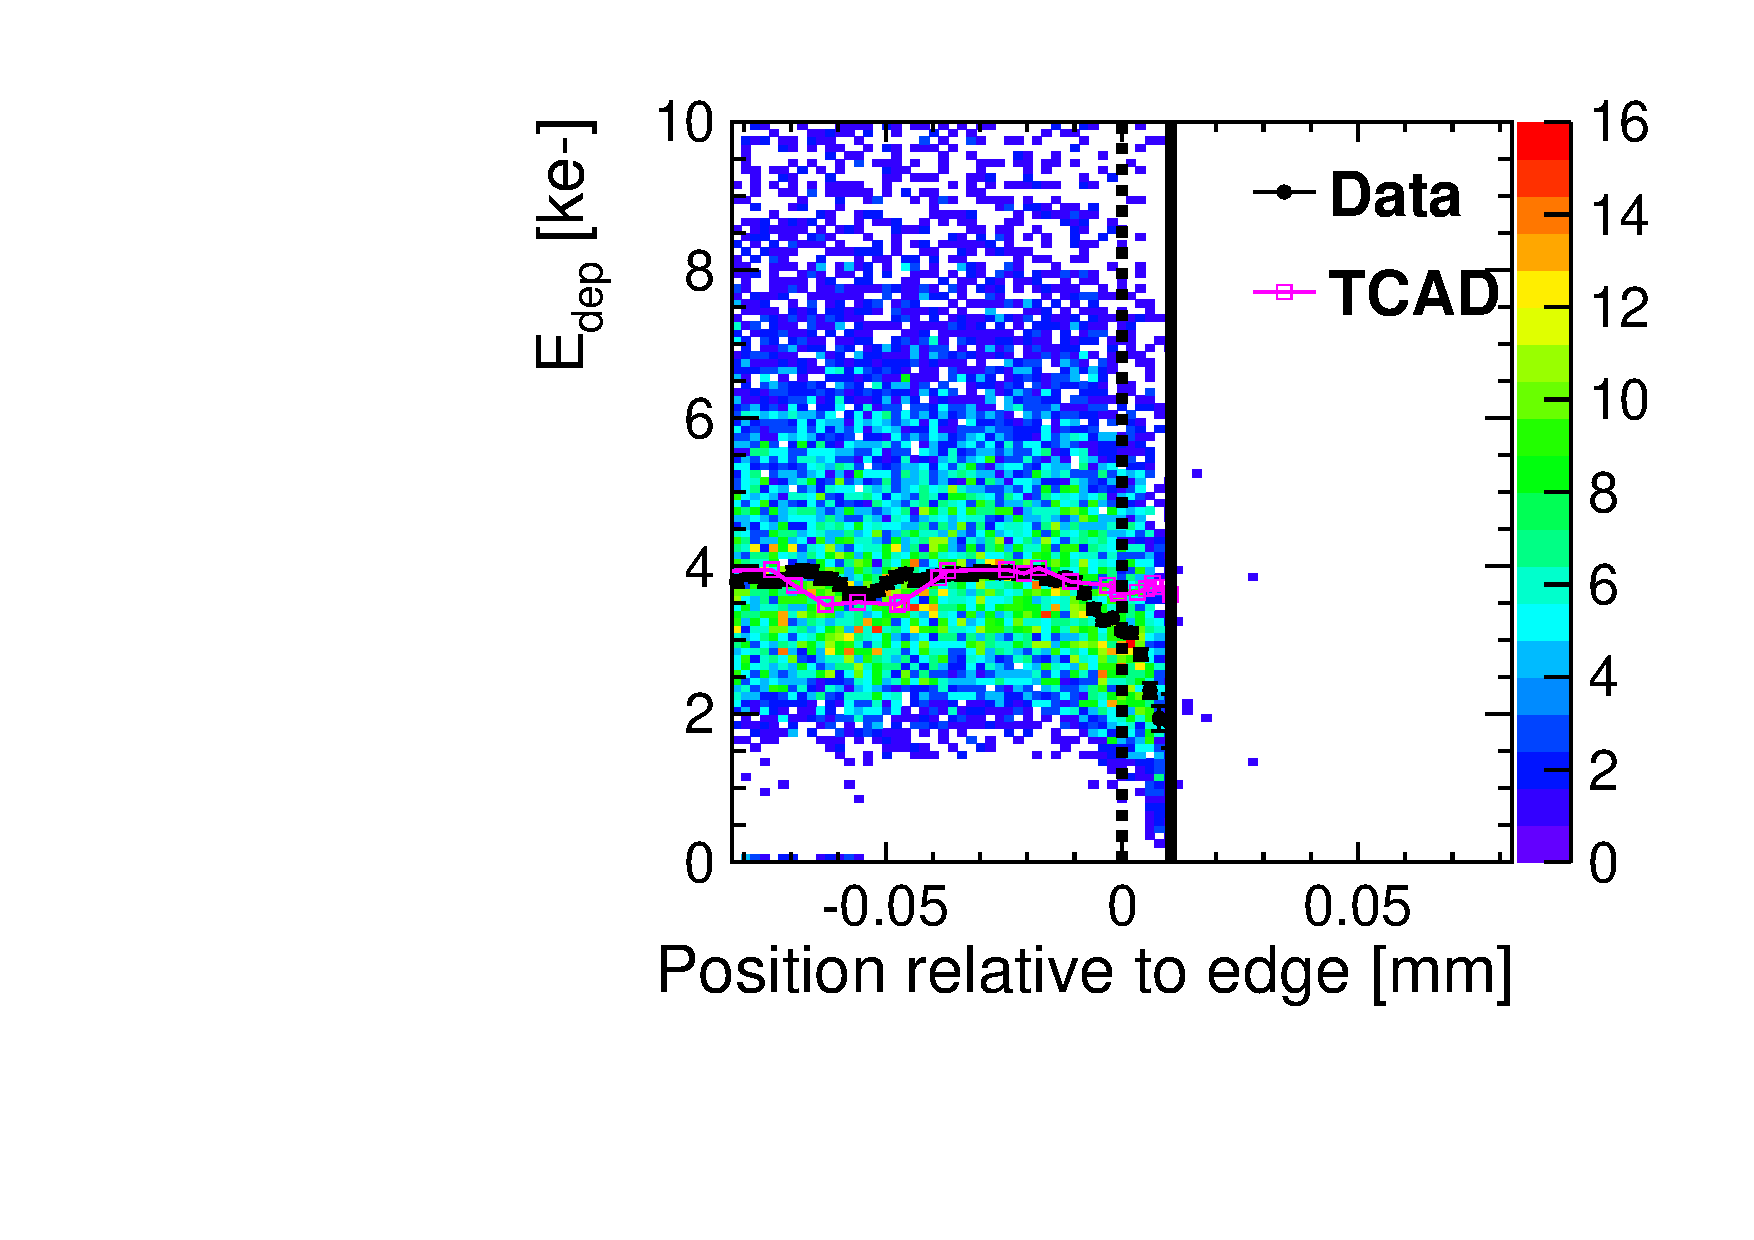
\includegraphics[width=\textwidth]{figures/ActiveEdge/23_FGR_Edep_TCAD_data.pdf}
    \caption{23-FGR-50}\label{fig:ChargeCollection23FGR}
  \end{subfigure}
  \caption{Charge collected as a function of the track position at the
    edge for the assemblies (a) 20-NGR-50 and (b) 23-FGR-50 in data
    and TCAD simulations. In data, only tracks within the central
    $40\%$ of the pixel cell area are considered.}
  \label{fig:ChargeCollectionNGRFGR}
\end{figure}



The grounded guard ring degrades significantly the detection
efficiency at the edge for thin sensors of $50\,\micron$. For
28-GNDGR-50, the efficiency drops in-between pixels as shown in
\cref{fig:EdgeEfficiency_28GNDGR50}. A large part of the charge is
collected by the guard ring. For the assembly with larger edge
distance (55-GNDGR-50), as shown in
\cref{fig:EdgeEfficiency_55GNDGR50}, the edge is not efficient
anymore.


For 28-GNDGR-50 and 55-GNDGR-50, both data and TCAD simulations show a
drop in the collected charge at the edge as shown in
\cref{fig:ChargeCollectionNGRFGR_50}. Most of the charge created in
the edge is collected by the guard ring.

\begin{figure}[htbp]
  \begin{subfigure}[b]{0.45\textwidth}
    \centering
    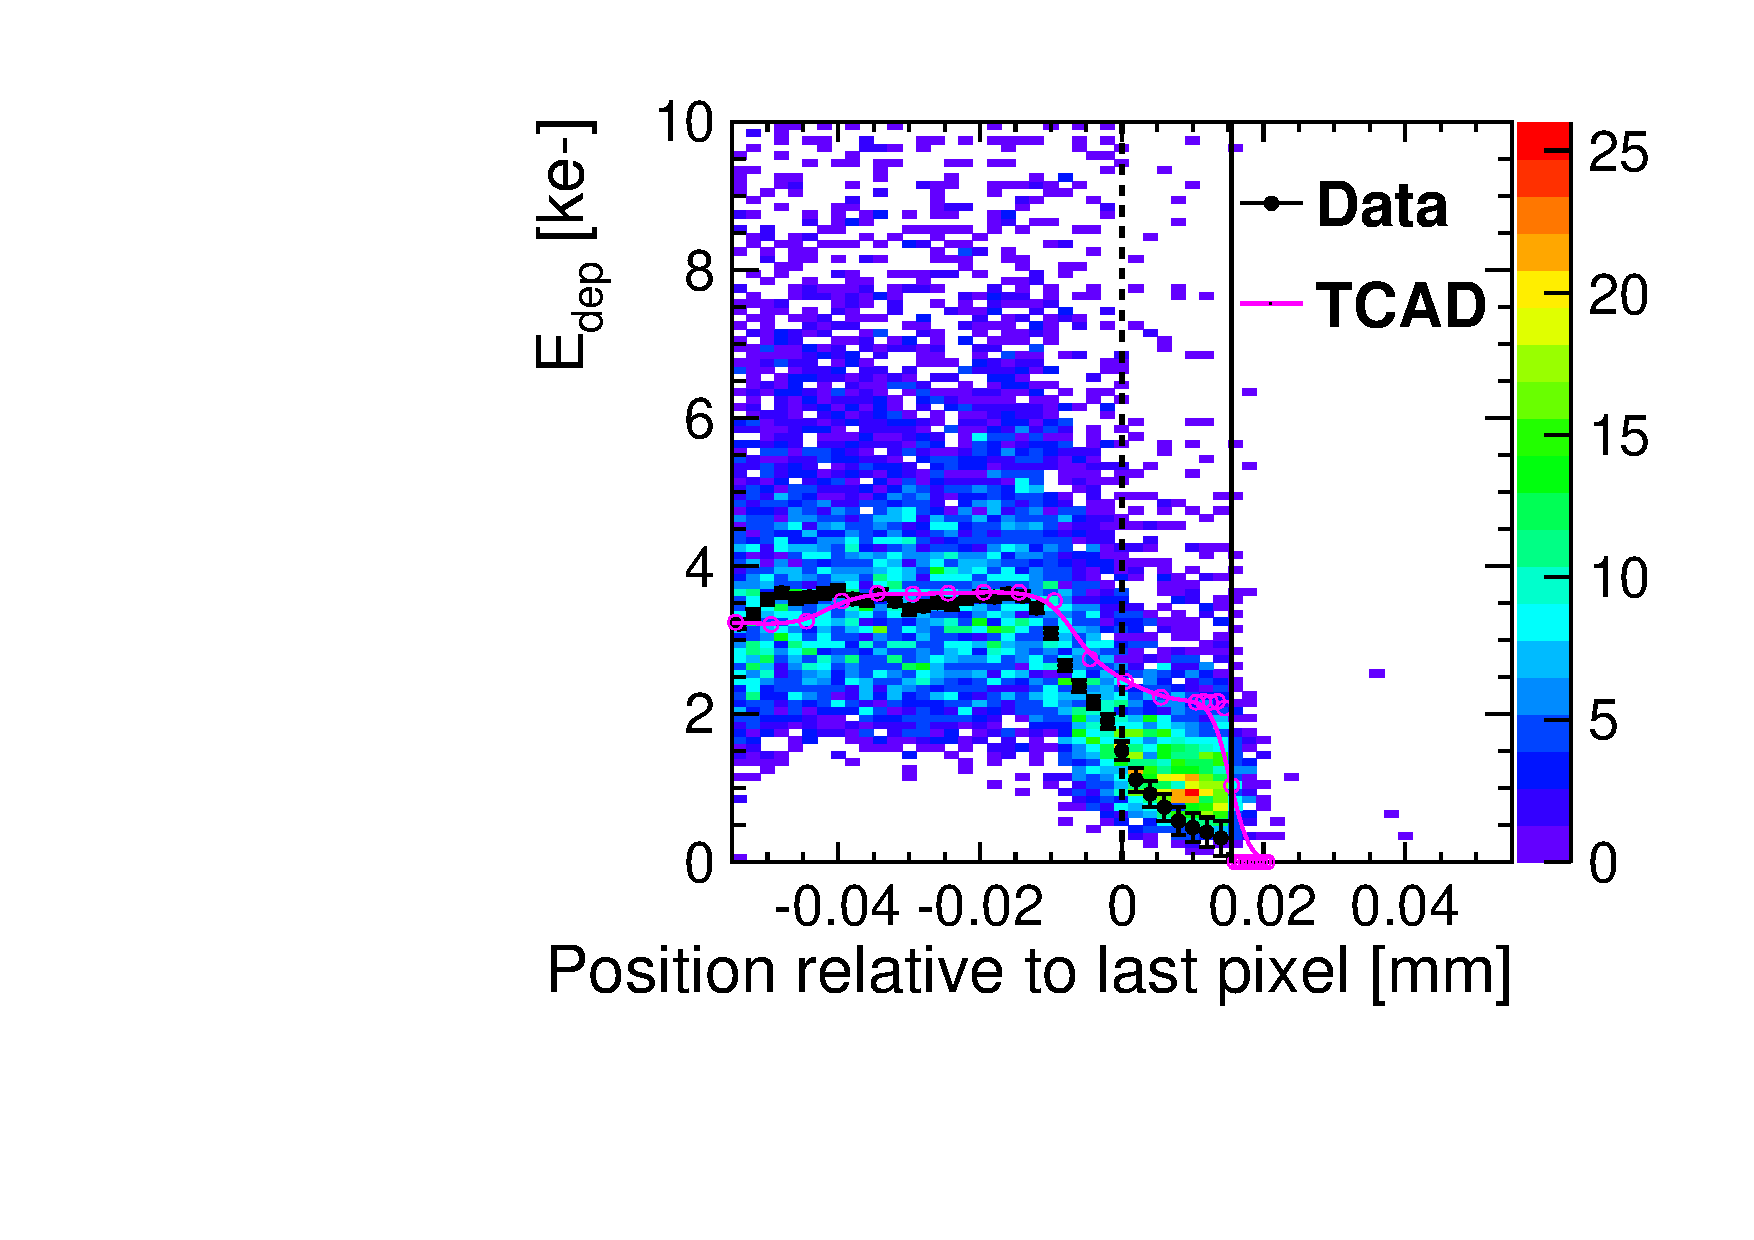
\includegraphics[width=\textwidth]{figures/ActiveEdge/28_GNDGR_Edep_TCAD_data.pdf}
    \caption{28-GNDGR-50}
  \end{subfigure}\hfill
  \begin{subfigure}[b]{0.45\textwidth}
    \centering
    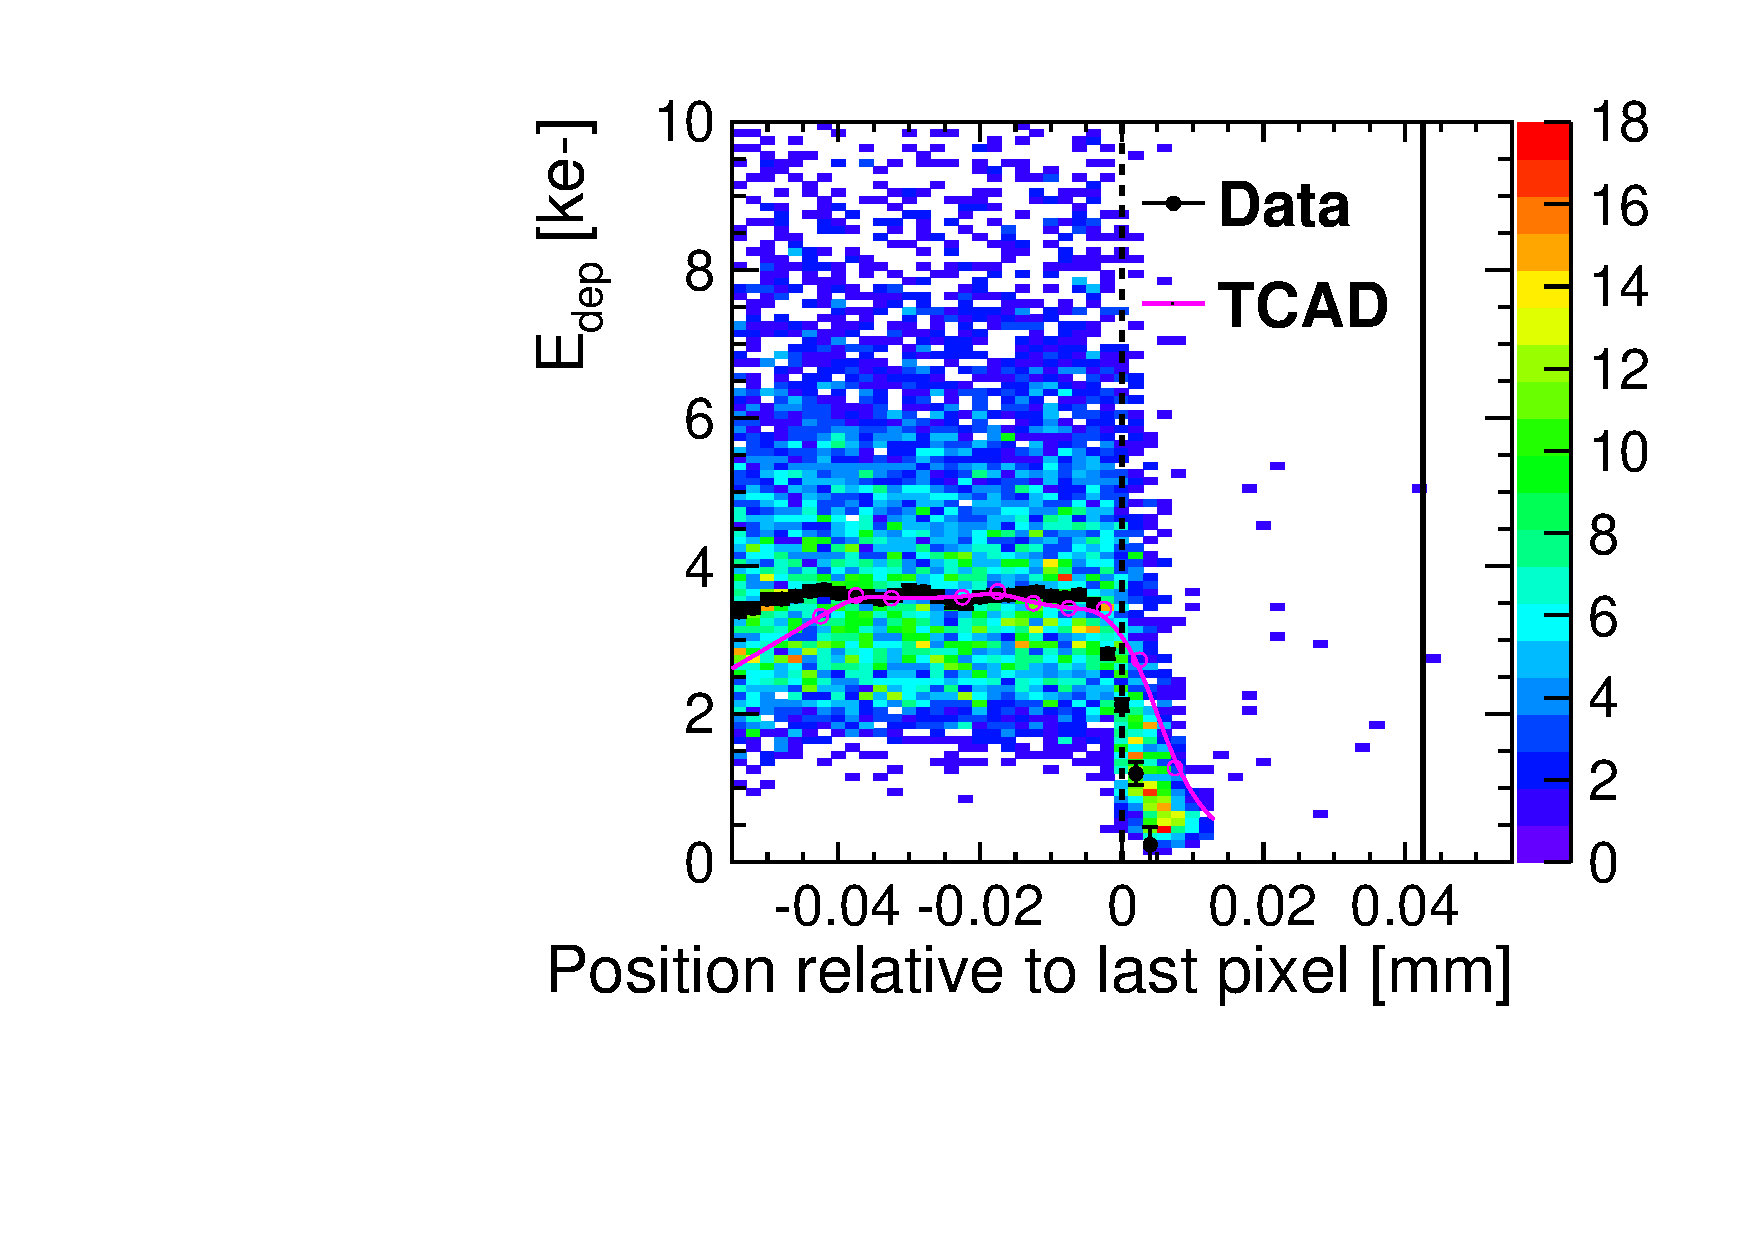
\includegraphics[width=\textwidth]{figures/ActiveEdge/55_GNDGR_Edep_TCAD_data.pdf}
    \caption{55-GNDGR-50}
  \end{subfigure}
  \caption{Charge collected as a function of the track position at the
    edge for the assemblies (a) 28-GNDGR-50 and (b) 55-GNDGR-50 in
    data and TCAD simulations. In data, only tracks within the central
    $7\%$ for 28-GNDGR-50 and $40\%$ for 55-GNDGR-50 of the pixel cell
    area are considered.}
  \label{fig:ChargeCollectionNGRFGR_50}
\end{figure}


Electric field streamlines define a family of curves tangent to the
velocity vector of the charge carrier
flow. \cref{fig:TCAD_streamlines} compares the distribution of the
streamlines in the edge for different configurations of guard rings in
TCAD simulations. The generated charge follows the streamlines and
gets collected by the implants. In the case where there is no guard
ring, all streamlines reach the first pixel. As confirmed by the data,
all the charge in the edge is collected without loss. In the case of a
floating guard ring, some streamlines reach the guard ring. This means
that some charge is lost in the guard ring instead of being collected
by the first pixel. Finally, in the case of a grounded guard ring,
more streamlines end up in the guard ring. This explains also the
larger drop in the collected charge and efficiency in the edge region.

\begin{figure}[htbp]
  \centering
  \begin{subfigure}[b]{0.45\textwidth}
    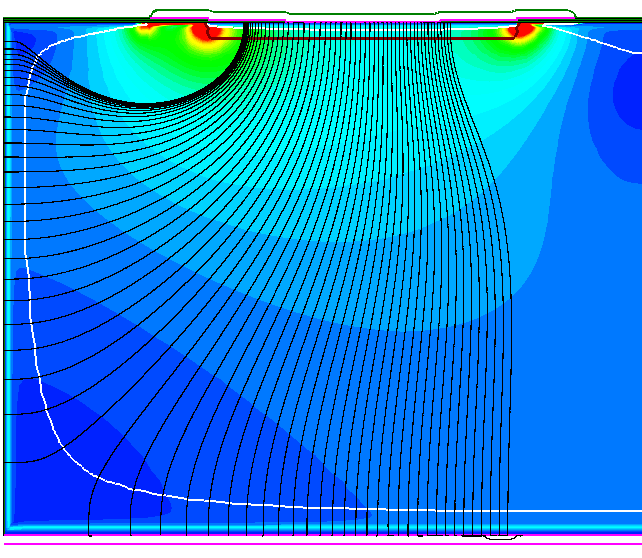
\includegraphics[width=0.8\textwidth]{figures/ActiveEdge/streamlines_20-NGR-50.png}
    \caption{20-NGR-50}
  \end{subfigure}\hfill
  \begin{subfigure}[b]{0.45\textwidth}
    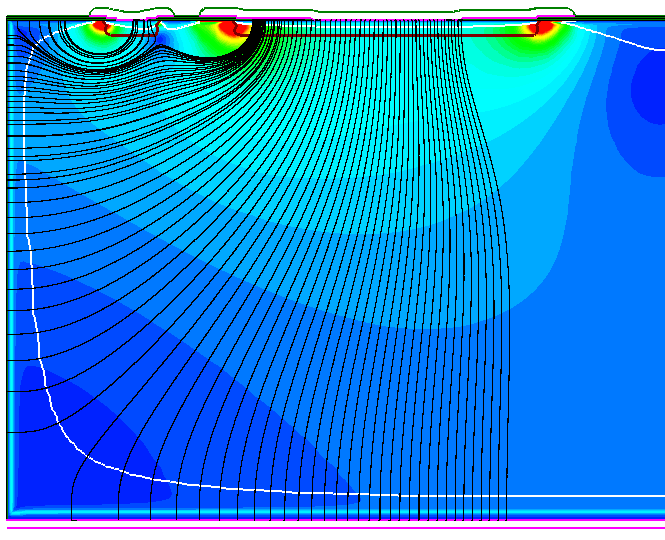
\includegraphics[width=0.8\textwidth]{figures/ActiveEdge/streamlines_23-FGR-50.png}
    \caption{23-FGR-50}
  \end{subfigure}\\
  \begin{subfigure}[b]{0.45\textwidth}
    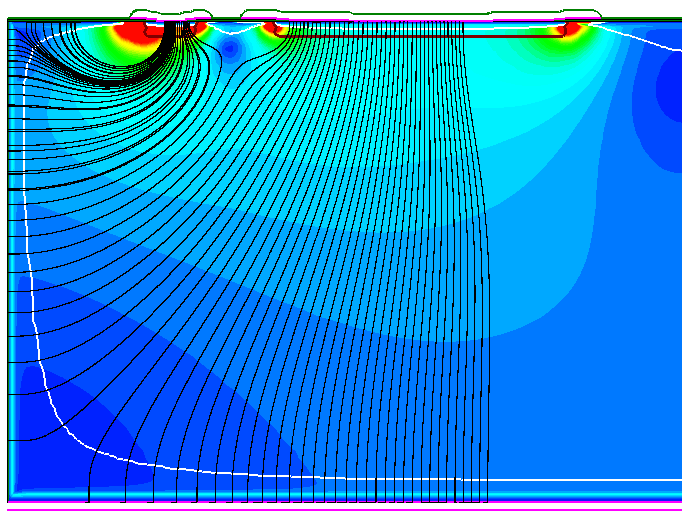
\includegraphics[width=0.8\textwidth]{figures/ActiveEdge/streamlines_28-GNDGR-50.png}
    \caption{28-GNDGR-50}
  \end{subfigure}\hfill
  \begin{subfigure}[b]{0.45\textwidth}
    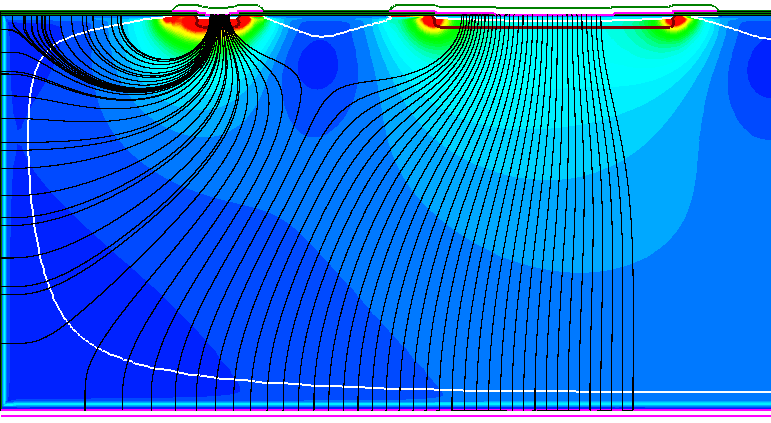
\includegraphics[width=\textwidth]{figures/ActiveEdge/streamlines_55-GNDGR-50.png}
    \caption{55-GNDGR-50}
  \end{subfigure}
  \caption{The electric field and the streamlines distributions for
    different configurations of guard ring for $50\,\micron$ thick
    sensors. The generated charges follow the streamlines. The
    depletion region is indicated by solid white lines.}
  \label{fig:TCAD_streamlines}
\end{figure}

For thin sensors, a floating guard ring appears to be the most
suitable solution, as it shows a high detection efficiency at the edge
and an acceptable breakdown behaviour.

%% --------------------------------------------- %%
\newpage
\subsection{The performance of $100\,\micron$ and $150\,\micron$ thick
  sensors}
\label{sec:EdgePerformance_100_150}

The assemblies 55-GNDGR-100 and 55-GNDGR-150 are efficient up to the
edge as shown in \cref{fig:EdgeEfficiency_100_150micron}. A slight
loss of the charge near the edge in data and simulations can be
observed for these assemblies as shown in
\cref{fig:ChargeCollectionThickGNDGR}. However, due to the large
amount of the ionisation charge, the signal does not drop below the
detection threshold and therefore the assembly remains efficient up to
the physical edge of the sensors.


\begin{figure}[htbp]
  \begin{subfigure}[b]{0.45\textwidth}
    \centering
    \includegraphics[width=\textwidth, page=15]{figures/TestBeam/edge_bcp.pdf}
    \caption{55-GNDGR-100}\label{fig:EdgeEfficiency_55GNDGR100}
  \end{subfigure}\hfill
  \begin{subfigure}[b]{0.45\textwidth}
    \centering
    \includegraphics[width=\textwidth, page=18]{figures/TestBeam/edge_bcp.pdf}
    \caption{55-GNDGR-150}\label{fig:EdgeEfficiency_55GNDGR150}
  \end{subfigure}
  \caption{The efficiency at the edge as a function of the positions
    for the assemblies having sensors with thicknesses of (a)
    $100\,\micron$ and (b) $150\,\micron$.}
  \label{fig:EdgeEfficiency_100_150micron}
\end{figure}

\begin{figure}[htbp]
  \begin{subfigure}[b]{0.45\textwidth}
    \centering
    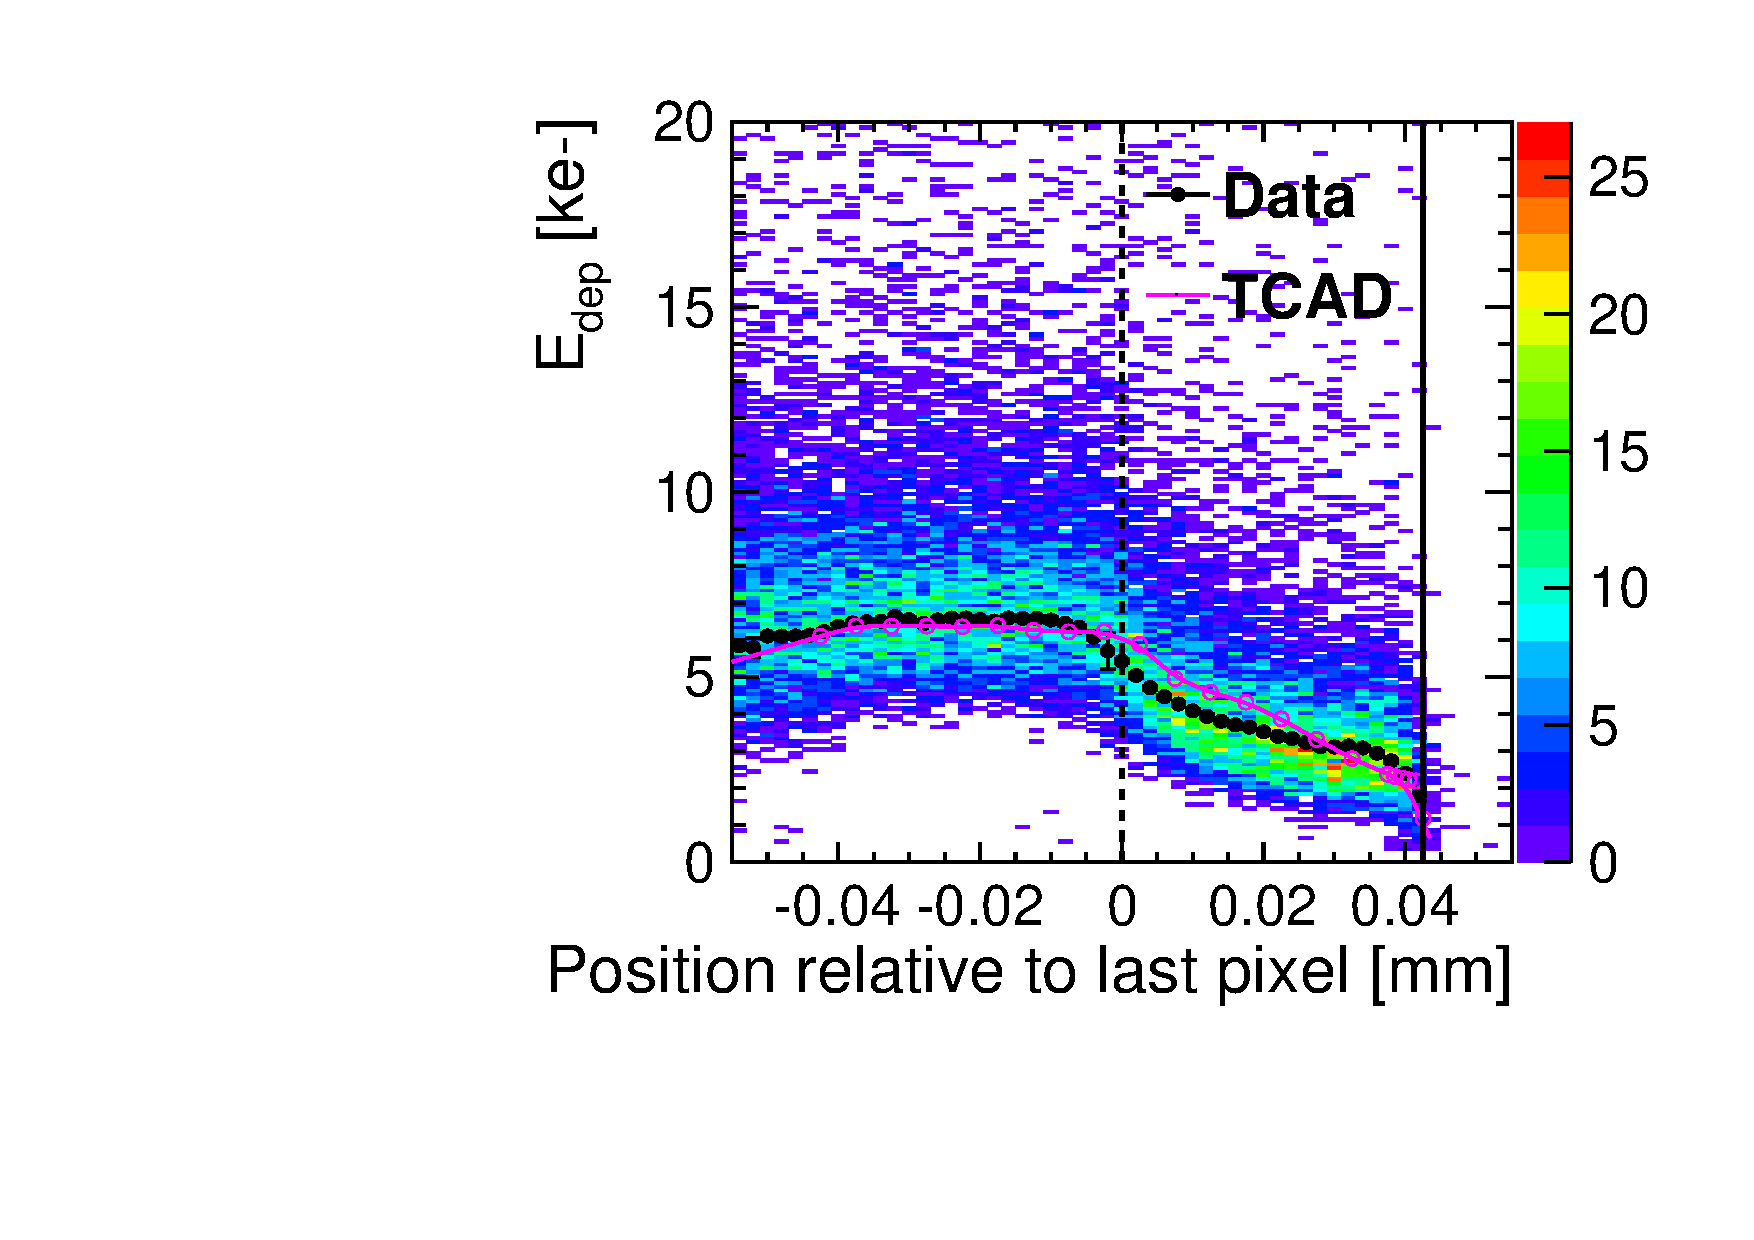
\includegraphics[width=\textwidth]{figures/ActiveEdge/55_GNDGR_100_Edep_TCAD_data.pdf}
  \caption{55-GNDGR-100}
  \end{subfigure}\hfill
  \begin{subfigure}[b]{0.45\textwidth}
    \centering
    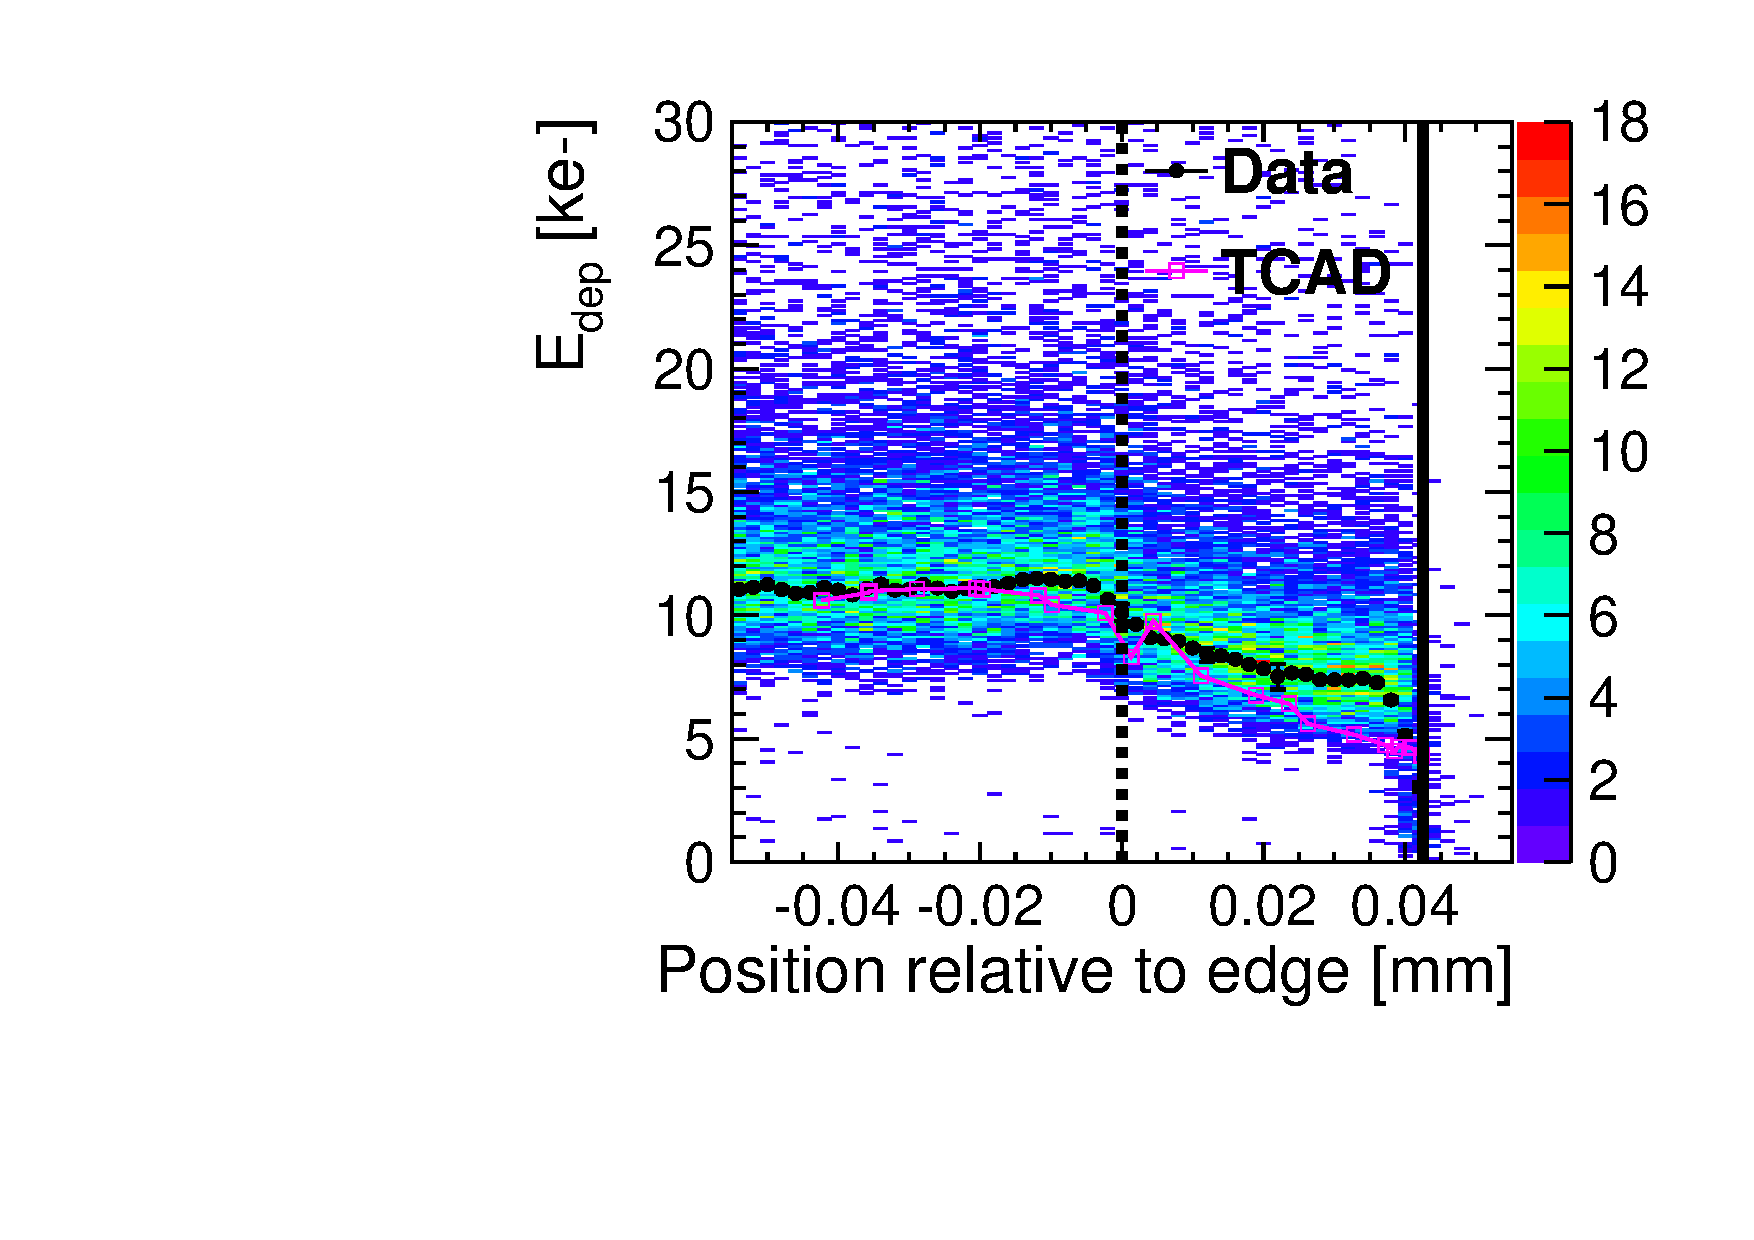
\includegraphics[width=\textwidth]{figures/ActiveEdge/55_GNDGR_150_Edep_TCAD_data.pdf}
  \caption{55-GNDGR-150}
  \end{subfigure}
  \caption{Charge collected as a function of the track position at the
    edge for the assemblies (a) 55-GNDGR-100 and (b) 55-GNDGR-150 in
    data and TCAD simulations. In data, only tracks within the central
    $40\%$ of the pixel cell area are considered.}
  \label{fig:ChargeCollectionThickGNDGR}
\end{figure}


For further investigation, \cref{fig:TCAD_streamlines_100_150} shows
the electric field and the streamline distributions for the
$100\,\micron$ and $150\,\micron$ thick sensors. For thicker devices,
some streamlines are reaching the guard ring but most of the charge is
collected by the pixels due to the thicker silicon bulk. The devices
remain still efficient up to $100\%$ even very close to the physical
edge. Therefore, for the thicker sensors of $100\,\micron$ and
$150\,\micron$, the grounded guard ring is a suitable solution.


\begin{figure}[htbp]
  \centering
  \begin{subfigure}[b]{0.45\textwidth}
    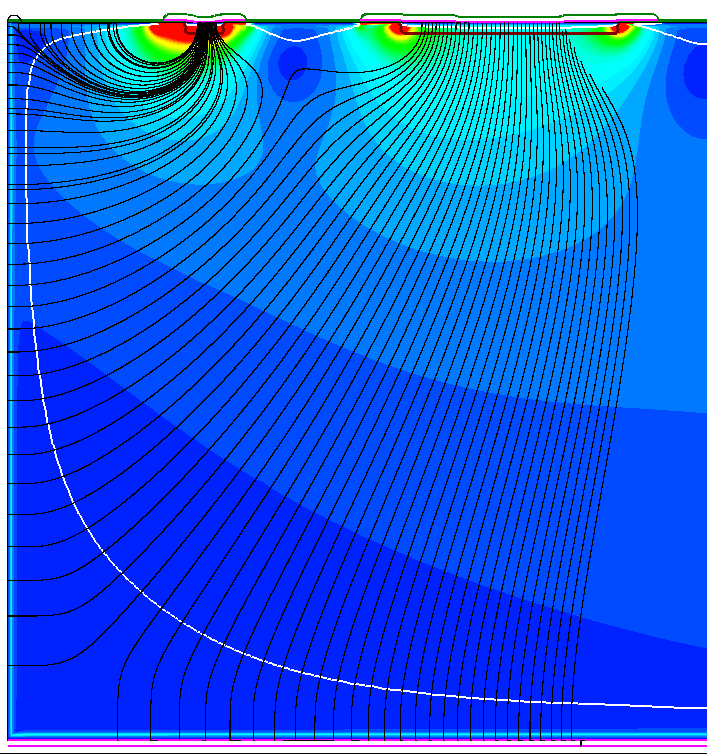
\includegraphics[width=0.8\textwidth]{figures/ActiveEdge/streamlines_55-GNDGR-100.png}
    \caption{55-GNDGR-100}
  \end{subfigure}\hfill
  \begin{subfigure}[b]{0.45\textwidth}
    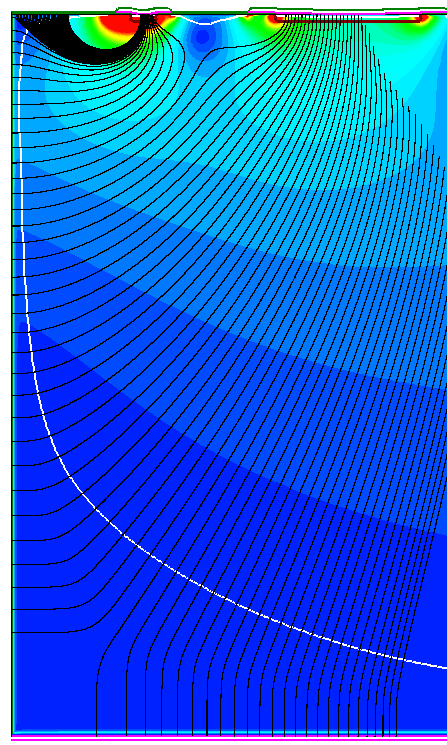
\includegraphics[width=0.8\textwidth]{figures/ActiveEdge/streamlines_55-GNDGR-150.png}
    \caption{55-GNDGR-150}
  \end{subfigure}
  \caption{The electric field and the streamlines distributions for
    different configurations of guard ring for $100\,\micron$ and
    $150\,\micron$ thick sensors. The generated charges follow the
    streamlines. The depletion region is indicated by solid white
    lines.}
  \label{fig:TCAD_streamlines_100_150}
\end{figure}




%% --------------------------------------------- %%
\newpage
\section{Summary}
\label{sec:summary_activeEdge}

\cref{fig:EdgeEff_2D} summarises the edge efficiency as a function of
the track position relative to the last pixel projected in one
direction for the different assemblies.

\begin{figure}[htbp]
  \centering
  %EdgeEfficiency_2D.py
  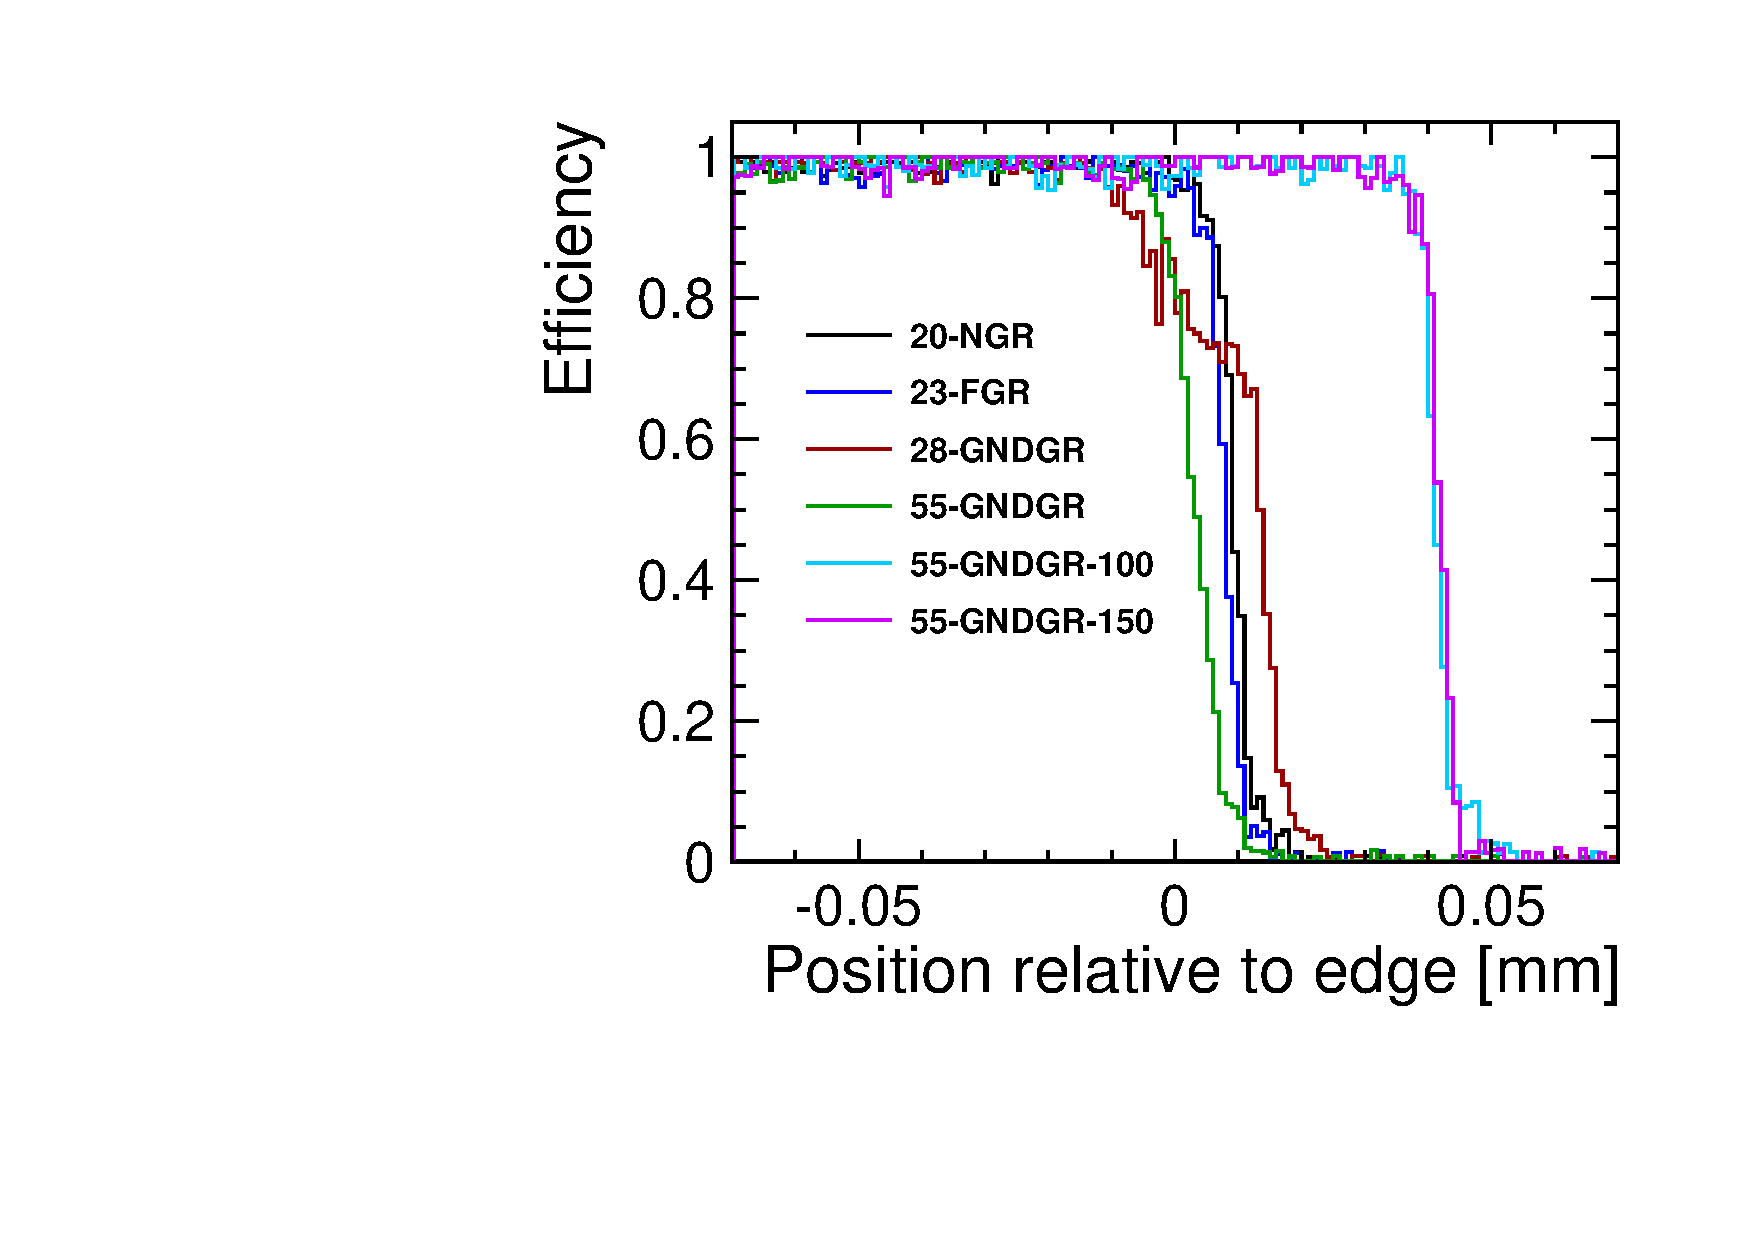
\includegraphics[width=0.7\textwidth]{figures/ActiveEdge/edgeEff_2D.pdf}
  \caption{The edge efficiency in data as a function of the track
    position relative to the edge projected in one direction.}
  \label{fig:EdgeEff_2D}
\end{figure}

For thin sensors ($50\,\micron$ thick), the grounded guard ring is not
a suitable solution since the guard ring collects most of the charge
in the edge and therefore lowers the efficiency. A floating guard ring
appears to be the most suitable solution, as it shows a high detection
efficiency at the edge and an acceptable breakdown behaviour.

For thicker sensors ($100\,\micron$ and $150\,\micron$), the grounded
guard ring is a suitable solution as a larger amount of charge is
deposited by the passage of MIP particles. Some of the deposited
charge is collected by the guard ring but these assemblies remain
efficient up to the physical edge.

The TCAD simulation model developed in this thesis for active edge
sensors is a powerful tool which allows to understand better the
functionality of these sensors. The simulations fulfill the
expectations for the operation of these devices: the floating guard
ring has the highest breakdown voltage since the guard ring smoothens
the potential drop between the physical edge and the first
pixel. However, for reproducing a simulation which would exactly
describe the loss of charge at the edge for a floating guard ring, the
capacitive coupling of the guard ring to all $\sim1000$ edge pixels is
needed to be taken into account.

%% The active-edge assembly with the floating guard ring shows an early
%% breakdown (almost like a grounded guard ring). This can be explained
%% by the fact that the guard-ring might be in touch with the last pixel
%% row in the Timepix3 which provides the ground potential and in reality
%% this guard ring might be grounded instead of being floating. Also,
%% this assembly shows more of charge loss at the edge than expected by
%% simulations.

In general, a good agreement between data and TCAD simulations is
observed. The discrepancies observed can be explained by the effects
not modeled in the simulations. The doping profiles used by the
manufacturer are not known for the TCAD simulations. This might affect
the electric field distribution inside the sensors. The depletion
region in simulations can therefore be slightly different than in
reality and therefore affecting the collected charge at the edge. The
energy loss fluctuations are also not considered in the
simulations. In addition, the Timepix3 chip has a non-linear behaviour
for low energy depositions. Therefore the quality of the calibration
also has an impact on the agreement between data and simulations
especially for low-energy depositions. Finally, the TCAD model is only
implemented in 2D and the coupling to other pixels and the sensor edge
is not fully simulated. A 3D simulation could help with a more precise
modeling of the capacitive coupling between the guard ring and the
neighbouring pixels.



% \newpage
% \section{Results temp}



% \begin{figure}[htbp]
%   \begin{subfigure}[b]{0.24\textwidth}
%     \centering
%     \includegraphics[width=\textwidth, page=5]{figures/TestBeam/edge_bcp.pdf}
%   \caption{}
%   \end{subfigure}\hfill
%   \begin{subfigure}[b]{0.24\textwidth}
%     \centering
%     \includegraphics[width=\textwidth, page=8]{figures/TestBeam/edge_bcp.pdf}
%   \caption{}
%   \end{subfigure}\hfill
%   \begin{subfigure}[b]{0.24\textwidth}
%     \centering
%     \includegraphics[width=\textwidth, page=11]{figures/TestBeam/edge_bcp.pdf}
%   \caption{}
%   \end{subfigure}\hfill
%   \begin{subfigure}[b]{0.24\textwidth}
%     \centering
%     \includegraphics[width=\textwidth, page=14]{figures/TestBeam/edge_bcp.pdf}
%   \caption{}
%   \end{subfigure}
%   \caption{}
%   \label{fig:ResultsTemp2}
% \end{figure}

% \begin{figure}[htbp]
%   \begin{subfigure}[b]{0.24\textwidth}
%     \centering
%     \includegraphics[width=\textwidth]{figures/ActiveEdge/20_NGR_TOT_edge.pdf}
%   \caption{}
%   \end{subfigure}\hfill
%   \begin{subfigure}[b]{0.24\textwidth}
%     \centering
%     \includegraphics[width=\textwidth]{figures/ActiveEdge/23_FGR_TOT_edge.pdf}
%   \caption{}
%   \end{subfigure}\hfill
%   \begin{subfigure}[b]{0.24\textwidth}
%     \centering
%     \includegraphics[width=\textwidth]{figures/ActiveEdge/28_GNDGR_TOT_edge.pdf}
%   \caption{}
%   \end{subfigure}\hfill
%   \begin{subfigure}[b]{0.24\textwidth}
%     \centering
%     \includegraphics[width=\textwidth]{figures/ActiveEdge/55_GNDGR_TOT_edge.pdf}
%   \caption{}
%   \end{subfigure}
%   \caption{}
%   \label{fig:ResultsTemp4}
% \end{figure}


% \begin{figure}[htbp]
%   \begin{subfigure}[b]{0.24\textwidth}
%     \centering
%     \includegraphics[width=\textwidth]{figures/ActiveEdge/20_NGR_Edep_TCAD_data.pdf}
%   \caption{}
%   \end{subfigure}\hfill
%   \begin{subfigure}[b]{0.24\textwidth}
%     \centering
%     \includegraphics[width=\textwidth]{figures/ActiveEdge/23_FGR_Edep_TCAD_data.pdf}
%   \caption{}
%   \end{subfigure}\hfill
%   \begin{subfigure}[b]{0.24\textwidth}
%     \centering
%     \includegraphics[width=\textwidth]{figures/ActiveEdge/28_GNDGR_Edep_TCAD_data.pdf}
%   \caption{}
%   \end{subfigure}\hfill
%   \begin{subfigure}[b]{0.24\textwidth}
%     \centering
%     \includegraphics[width=\textwidth]{figures/ActiveEdge/55_GNDGR_Edep_TCAD_data.pdf}
%   \caption{}
%   \end{subfigure}
%   \caption{}
%   \label{fig:ResultsTemp5}
% \end{figure}





% \begin{figure}[htbp]
%   \begin{subfigure}[b]{0.45\textwidth}
%     \centering
%     \includegraphics[width=\textwidth, page=15]{figures/TestBeam/edge_bcp.pdf}
%   \caption{}
%   \end{subfigure}\hfill
%   \begin{subfigure}[b]{0.45\textwidth}
%     \centering
%     \includegraphics[width=\textwidth, page=18]{figures/TestBeam/edge_bcp.pdf}
%   \caption{}
%   \end{subfigure}
%   \caption{}
%   \label{fig:ResultsTemp6}
% \end{figure}



% \begin{figure}[htbp]
%   \begin{subfigure}[b]{0.45\textwidth}
%     \centering
%     \includegraphics[width=\textwidth]{figures/ActiveEdge/55_GNDGR_100_Edep_TCAD_data.pdf}
%   \caption{}
%   \end{subfigure}\hfill
%   \begin{subfigure}[b]{0.45\textwidth}
%     \centering
%     \includegraphics[width=\textwidth]{figures/ActiveEdge/55_GNDGR_150_Edep_TCAD_data.pdf}
%   \caption{}
%   \end{subfigure}
%   \caption{}
%   \label{fig:ResultsTemp7}
% \end{figure}


% \begin{figure}[htbp]
%   \begin{subfigure}[b]{0.45\textwidth}
%     \centering
%     \includegraphics[width=\textwidth]{figures/ActiveEdge/55_GNDGR_100_TOT_edge.pdf}
%   \caption{}
%   \end{subfigure}\hfill
%   \begin{subfigure}[b]{0.45\textwidth}
%     \centering
%     \includegraphics[width=\textwidth]{figures/ActiveEdge/55_GNDGR_150_TOT_edge.pdf}
%   \caption{}
%   \end{subfigure}
%   \caption{}
%   \label{fig:ResultsTemp8}
% \end{figure}






%% %%%%%%%%%%%%%%%%%%%%
%% \begin{figure}[htbp]
%%   \begin{subfigure}[b]{0.45\textwidth}
%%     \centering
%%     \includegraphics[width=\textwidth, page=15]{figures/TestBeam/edge_bcp.pdf}
%%   \caption{}
%%   \end{subfigure}\hfill
%%   \begin{subfigure}[b]{0.45\textwidth}
%%     \centering
%%     \includegraphics[width=\textwidth, page=18]{figures/TestBeam/edge_bcp.pdf}
%%   \caption{}
%%   \end{subfigure}
%%   \caption{}
%%   \label{fig:ResultsTemp4}
%% \end{figure}

%% \begin{figure}[htbp]
%%   \begin{subfigure}[b]{0.45\textwidth}
%%     \centering
%%     \includegraphics[width=\textwidth, page=17]{figures/TestBeam/edge_bcp.pdf}
%%   \caption{}
%%   \end{subfigure}\hfill
%%   \begin{subfigure}[b]{0.45\textwidth}
%%     \centering
%%     \includegraphics[width=\textwidth, page=20]{figures/TestBeam/edge_bcp.pdf}
%%   \caption{}
%%   \end{subfigure}
%%   \caption{}
%%   \label{fig:ResultsTemp5}
%% \end{figure}

%% \begin{figure}[htbp]
%%   \begin{subfigure}[b]{0.45\textwidth}
%%     \centering
%%     \includegraphics[width=\textwidth]{figures/ActiveEdge/TCAD_data_Edep_55_GNDGR_100.pdf}
%%   \caption{}
%%   \end{subfigure}\hfill
%%   \begin{subfigure}[b]{0.45\textwidth}
%%     \centering
%%     \includegraphics[width=\textwidth]{figures/ActiveEdge/TCAD_data_Edep_55_GNDGR_150.pdf}
%%   \caption{}
%%   \end{subfigure}
%%   \caption{}
%%   \label{fig:ResultsTemp6}
%% \end{figure}


%%%%%%%%%%%%%%%%%%%%%%%%%%%%%%%%%%%
% \begin{figure}[htbp]
%   \centering
%   \begin{minipage}[t]{.4\textwidth}
%     \centering
%     \vspace{0pt}
%     \includegraphics[width=0.95\textwidth]{figures/ActiveEdge/pixelLayout_withLayers.png}
%     \caption{}
%     \label{fig:PixelLayout}
%   \end{minipage}
%   \hfill
%   \begin{minipage}[t]{.56\textwidth}
%     \centering
%     \vspace{0pt}
%     \captionof{table}{Layers and dimensions from the gds geometry
%       (taken from Timepix 20um GR FLOAT).}
%     \label{tab:PixelStackDimensions}
%     \begin{tabular}{l c c}
%       \toprule
%       Layer number & Layer & Diameter [\micron]\\
%       \midrule
%       6 & metal & 36 \\
%       3 & - & 34.62 \\
%       8 & implant & 30 \\
%       9 & UBM (for thin film lift off metal) (??) & 25.6 \\
%       15 & passivation & 19.5 \\
%       5 & contact to connect Al to Si & 15 \\
%       \bottomrule
%     \end{tabular}
%   \end{minipage}
% \end{figure}




% \begin{figure}[htbp]
%   \centering
%   \begin{subfigure}[b]{0.33\textwidth}
%     \centering
%     \fbox{\includegraphics[width=0.95\textwidth]{figures/ActiveEdge/20umEdge_float_GR_withText.png}}
%     \caption{20~\micron edge: Floating guard ring}
%     \label{fig:GuardRingLayout_20_float_GR}
%   \end{subfigure}\hfill
%   \centering
%   \begin{subfigure}[b]{0.33\textwidth}
%     \centering
%     \fbox{\includegraphics[width=0.95\textwidth]{figures/ActiveEdge/20umEdge_GND_GR_withText.png}}
%     \caption{20~\micron edge: GND guard ring}
%     \label{fig:GuardRingLayout_20_GND_GR}
%   \end{subfigure}\hfill
%   \centering
%   \begin{subfigure}[b]{0.33\textwidth}
%     \centering
%     \fbox{\includegraphics[width=0.95\textwidth]{figures/ActiveEdge/50umEdge_GND_GR_withText.png}}
%     \caption{50~\micron edge: GND guard ring}
%     \label{fig:GuardRingLayout_50_GND_GR}
%   \end{subfigure}
%   \label{fig:GuardRingLayout}
% \end{figure}


% For the 50~\micron grounded GR, the dimensions of the pixels are
% differente from above.
% \captionof{table}{Layers and dimensions from the gds geometry
%   (taken from Timepix 20um GR FLOAt and from Timepix 50~\micron grounded GR).}
% \label{tab:PixelStackDimensions}
% \begin{tabular}{l c c c}
%   \toprule
%   Layer number & Layer & Diameter (20 float) [\micron] & Diameter (50 GND) [\micron]\\
%   \midrule
%   6 & metal & 36 & 40 \\
%   3 & - & 34.62 & 36 \\
%   8 & implant & 30 & 30 \\
%   9 & UBM & 25.6 & 25.6 \\
%   15 & passivation & 19.5 & 19.5 \\
%   5 & contact to connect Al to Si & 15 & 15 \\
%   \bottomrule
% \end{tabular}






% For the $50\,\micron$ thick sensors, 4 edge configurations are
% studied: 
% \begin{itemize}
% \item 20-NGR does not contain any guard-ring in the edge with an edge
%   distance of $20\,\micron$.
% \item 23-FGR contains a guard ring with a floating potential. The
%   edge distance is $23\,\micron$.
% \item 28-GNDGR contains a guard ring connected to the ground potential
%   with an edge distance of $28\,\micron$.
% \item 55-GNDGR contains a guard ring connected to the ground potential
%   with an edge distance of $55\,\micron$.
% \end{itemize}

% For 55-GNDGR-100 ($100\,\micron$ thick sensor) and 55-GNDGR-150
% ($150\,\micron$ thick sensor), the edge contains a guard ring
% connected to the ground potential with an edge distance of
% $55\,\micron$.

% \begin{table}[htbp]
%   \centering
%   \caption{Advacam active-edge n-in-p planar pixel sensor assemblies. The edge distance is defined by the distance between the last pixel implant and the physical sensor edge.}
%   \label{tab:activeEdgeAssembliesList}
%   \begin{tabular}{lccc}
%     \toprule
%     Assembly & Thickness [\micron] & Edge distance [\micron] & ID \\
%     \midrule
%     20-NGR  & 50 & 20 & W19\_G7 \\
%     23-FGR & 50 & 23 & W19\_F7 \\
%     28-GNDGR & 50 & 28 & W19\_L8 \\
%     55-GNDGR & 50 & 55 &W19\_C7 \\ \hline
%     55-GNDGR-100 & 100 & 55 & W5\_E2  \\ \hline
%     55-GNDGR-150 & 150 & 55 & W5\_F1 \\
%     \bottomrule
%   \end{tabular}
% \end{table}
